\documentclass{beamer}
%\documentclass[draft]{beamer}
%\documentclass[handout]{beamer}
%\documentclass[draft,handout]{beamer}

\usepackage[brazil]{babel}
\usepackage[latin1]{inputenc}
\usepackage[T1]{fontenc}
\usepackage{type1ec}
\usepackage{graphicx}
\usepackage{multirow}
\usepackage{soul}
\usepackage{ifpdf}

\ifpdf
	\usepackage{epstopdf}
\fi

%\let\newfloat=\undefined
\usepackage[portugues,boxed]{algorithm2e}
\usepackage{algorithmic}

%\newcommand{\theHalgorithm}{\arabic{algorithm}}

% Mudando o label dos algoritmos para portug�s
%\floatname{algorithm}{Algoritmo}

% Vari�veis matem�ticas
\newcommand{\C}{\mathcal{C}}
\newcommand{\Cl}{\mathcal{C}^{'}}
\newcommand{\D}{\mathcal{D}}
\newcommand{\Dl}{\mathcal{D}^{'}}
\newcommand{\Dlc}{\mathcal{D}^{'}_c}
\newcommand{\F}{\mathcal{F}}
\newcommand{\Fl}{\mathcal{F}^{'}}
\newcommand{\Flc}{\mathcal{F}^{'}_c}
\newcommand{\Fli}{\mathcal{F}^{'}_i}
\newcommand{\Flt}{\mathcal{F}^{'}_t}
\newcommand{\G}{\mathcal{G}}
\newcommand{\I}{\mathcal{I}}
\newcommand{\Il}{\mathcal{I}^{'}}
\newcommand{\M}{\mathcal{M}}
\newcommand{\Or}{\mathcal{O}}
\newcommand{\R}{\mathcal{R}}
%\newcommand{\Se}{\mathcal{S}}

\usetheme[compress]{Berlin}
%\usetheme{Berlin}

\title[Minera��o de Padr�es Freq�entes e Ortogonais]{Minera��o de Padr�es Freq�entes Ortogonais e sua Aplica��o em Classifica��o Associativa}
\author[Leandro S. Costa]{Leandro Souza Costa \\ Orientador: Wagner Meira Jr.}
\institute[DCC-UFMG]{Departamento de Ci�ncia da Computa��o \\ Universidade Federal de Minas Gerais}
\logo{
\includegraphics[height=.8cm]{../thesis/img/speed}}
\date[Disserta��o de Mestrado]{Defesa de Disserta��o de Mestrado \\ \today}

\begin{document}

\setbeamercovered{transparent}

\begin{frame}
\titlepage
\end{frame}

%\section*{Sum�rio}
%\begin{frame}[shrink=5]
%\tableofcontents
%\end{frame}

\chapter{Introdu��o}
\label{chapter:introducao}

H� muito j� n�o � mais novidade o fato de que vivemos, hoje, na chamada \textbf{Era da Informa��o} (termo cunhado por Daniel Bell, professor em�rito da Universidade de Harvard), que se define pelo r�pido desenvolvimento da tecnologia de informa��o, caracter�stica marcante da \textbf{Sociedade P�s-Industrial}, onde nota-se que, mais importante que possuir a informa��o, � saber onde e como encontr�-la.
\par
Ao longo dos �ltimos anos, o desenvolvimento tecnol�gico fez com que o constante armazenamento de dados se tornasse uma atividade f�cil e barata. A conseq��ncia deste fato foi a alimenta��o de enormes bases de dados, o que proporcionou a  necessidade de se pensar em novas solu��es de ger�ncia, manuten��o e, posteriormente, acesso.
\par
Os Sistemas de Gerenciamento de Banco de Dados (\textbf{SGBD}) surgiram como uma solu��o para ger�ncia e manuten��o de bases, com o objetivo de retirar da aplica��o cliente a responsabilidade de gerenciar o acesso, a manipula��o e a organiza��o dos dados. Entretanto, embora os complexos SGBD's tenham se consolidado como eficientes sistemas na ger�ncia de complexos volumes de dados, e tratado com efic�cia a recupera��o de informa��es em grandes cole��es, da exist�ncia de tais bases surgiu a necessidade de m�todos mais avan�ados de recupera��o de informa��o, como redu��o de volume de dados, extra��o da ess�ncia da informa��o armazenada, descoberta de padr�es, dentre outros.
\par
Como resposta � necessidade dos novos m�todos de recupera��o de informa��o, surgiu o que chamamos hoje de \textbf{Minera��o de Dados}.

\section{Minera��o de Dados}

Minera��o de dados � o resultado de um longo processo de pesquisa e desenvolvimento, considerado uma das mais importantes fronteiras entre bases de dados e sistemas de informa��o, e um dos mais promissores desenvolvimentos interdisciplinares na tecnologia da informa��o \citep{Han00}. Podemos defini-la como o conjunto de m�todos n�o triviais de an�lise de dados e extra��o de informa��o potencialmente �til, impl�cita, previamente desconhecida, e suas novas formas de representa��o e visualiza��o \citep{Kumar06, Hand01, PiatetskyF91}.
\par
O termo Minera��o de Dados � freq�entemente mencionado no contexto de \textbf{Descoberta de Conhecimento em Bases de Dados} (\textbf{KDD - \textit{Knowledge Discovery in Databases}}), definido como um processo de extra��o de conhecimentos v�lidos, novos, potencialmente �teis e compreens�veis para apoiar a tomada de decis�o \citep{Fayyad96}. Para tanto, o KDD faz uso de diversos artif�cios, incluindo m�todos estat�sticos, reconhecimento de padr�es, visualiza��o, banco de dados, aprendizado de m�quia, intelig�ncia artificial, \textit{data warehouse}, dentre outros \citep{Sassi06}.
\par
O processo de descoberta de conhecimento em bases de dados consiste na seguinte seq��ncia de etapas:

\begin{enumerate}
	\item{Aprendizado:} Entendimento do dom�nio da aplica��o, que inclui conhecimento pr�vio da aplica��o e dos seus objetivos;
	\item{Sele��o:} Coleta dos dados, constitu�do pela defini��o de uma base de dados e pela sele��o de um conjunto (ou sub-conjunto) de dados e atributos a serem considerados;
	\item{Pr�-processamento:} Abrange execu��o de opera��es b�sicas como remo��o de ru�dos, defini��o de procedimentos e estrat�gias aplic�veis a dados faltosos, decis�es relacionadas a tipos de dados, dentre outras tarefas;
	\item{Transforma��o:} Consiste na defini��o de atributos indicados para representar os dados, defini��o da dimensionalidade dos dados, e outros m�todos de transforma��o para reduzir o n�mero de vari�veis sob considera��o;
	\item{Minera��o de Dados:} Inclui a escolha da fun��o de minera��o de dados, de acordo com o prop�sito do modelo (podendo ser classifica��o, agrupamento, sumariza��o, etc.), e do algoritmo a ser aplicado, que depende de decis�es como qual modelo � mais apropriado considerando-se a natureza dos dados. Por exemplo, modelos para dados categ�ricos s�o diferentes de modelos para dados cont�nuos. A execu��o da minera��o de dados se resume em pesquisar por padr�es de interesse numa representa��o (ou conjunto de representa��es) definida de acordo com a fun��o de minera��o de dados escolhida;
	\item{Interpreta��o e Avalia��o:} Esta etapa pode resultar no retorno a qualquer um dos passos anteriores, caso os resultados n�o sejam satisfat�rios, e alguma altera��o seja necess�ria para a sua melhoria;
	\item{Utiliza��o do Conhecimento:} Consiste na incorpora��o do conhecimento adquirido promovendo a��es ou simplesmente documentando e reportando resultados para as partes de interesse.
\end{enumerate}

De acordo com \cite{Fayyad96}, minera��o de dados � um passo do processo KDD que consiste na enumera��o de padr�es sobre os dados, sujeito a aceit�veis limita��es de efici�ncia computacional. Considerando que padr�es enumer�veis sobre uma base finita de dados s�o potencialmente infinitos, e que tal enumera��o envolve alguma forma de pesquisa num espa�o amplo, limita��es computacionais adicionam severos limites sobre o sub-espa�o que pode ser explorado por um algoritmo de minera��o de dados. Por este motivo, a constante busca por novas metodologias e algoritmos de enumera��o de padr�es em grandes bases de dados t�m sido foco de in�meras frentes de pesquisa em minera��o de dados.

%\par
%A princ�pio, minera��o de dados � uma t�cnica que pode ser aplicada a quaisquer tipos de dados, incluindo dados de transa��es, \textit{multimedia}, dados espaciais, informa��es temporais, e at� mesmo a \textbf{WWW} (\textit{World Wide Web}). Os tipos de padr�es que podem se descobertos dependem das funcionalidades aplicadas. As funcionalidades de minera��o de dados e a variedade de conhecimento que elas podem descobrir s�o apresentadas na seguinte lista:

%\begin{itemize}
%	\item{Caracteriza��o:} Categoriza��o de dados
%\end{itemize}
%
%Que tipo de dado pode ser minerado?
%\par
%O que pode ser descoberto?
%\par
%Tudo o que pode ser descoberto � de interesse do usu�rio?
%\par
%Como sistemas de minera��o de dados podem ser categorizados?
%\par
%What are the "issues"?
%\par
%Falar das solu��es encontradas na minera��o de dados para resolver os problemas citados, (agrupamento, regras associativas, etc). "Minera��o de dados � uma tecnologia usada para revelar informa��o estrat�gica escondida em grandes massas de dados". \\
%fonte: http://br.geocities.com/dugimenes/mineracao.htm \\
%fonte: http://pt.wikipedia.org/wiki/Minera\%C3\%A7\%C3\%A3o\_de\_dados \\
%Citar \cite{Kumar06}. \\
%Procurar livros, como \cite{Han00}. \\
%http://books.google.com/books?hl=en\&lr=\&id=AfL0t-YzOrEC\&oi=fnd\&pg=PR21\&dq=data+mining\&ots=UuSVuVarG6\&sig=swJzbDeqSGlffWudUjXszg5vNPA\#PPP1,M1

\subsection{Padr�es Freq�entes}

De acordo com \cite{Han00}, padr�es freq�entes s�o padr�es que aparecem freq�entemente num conjunto de dados. Por exemplo, um conjunto de itens, como ``caf�'' e ``leite'', que aparecem juntos com freq��ncia em transa��es de uma base de dados, � considerado um padr�o freq�ente. Uma seq��ncia, como comprar uma c�mera fotogr�fica, e logo depois um cart�o de mem�ria, se ocorre freq�entemente na base de dados de um estabelecimento comercial, tamb�m � considerada um padr�o freq�ente.
\par
Padr�es freq�entes assumem um papel essencial em muitas tarefas de minera��o de dados que possuem, como objetivo, encontrar padr�es de determinado interesse numa base, tais como regras de associa��o, correla��es, seq��ncias, epis�dios, classificadores, agrupamentos e muitas outras das quais a minera��o de regras de associa��o � uma das mais populares \citep{goethals03survey}. Desde a introdu��o deste termo, em 1993, por \citeauthor{agrawal93mining}, a minera��o de padr�es freq�entes e regras de associa��o t�m recebido grande aten��o. Nas �ltimas d�cadas, centenas de artigos cient�ficos foram publicados apresentando algoritmos, abordagens e melhorias para resolver os problemas de minera��o de padr�es freq�entes e regras de associa��o de forma mais eficiente.
\par
Dentre as caracter�sticas mais importantes dos padr�es freq�entes, podemos citar o suporte, que representa a medida de popularidade do padr�o em rela��o � base. Um padr�o � considerado freq�ente se possui suporte maior que um dado limite inferior. Na pr�tica, n�o estamos interessados apenas no conjunto de padr�es freq�entes, mas tamb�m nos respectivos suportes destes padr�es.

%�timo Survey sobre minera��o de padr�es freq�entes (possui descri��o do problema, minera��o de itemsets, espa�o de busca, regras de associa��o, algoritmo apriori fp-growth, etc...): \cite{goethals03survey}.

\subsection{Regras de Associa��o}

Em minera��o de dados, regras de associa��o s�o utilizadas para descobrir elementos que co-ocorrem freq�entemente numa determinada base de dados. A motiva��o por tr�s deste tema est� relacionada com a grande quantidade de aplica��es poss�veis de se construir com o aux�lio de regras de associa��o, como por exemplo, quest�es relacionadas ao comportamento de clientes num determinado estabelecimento comercial.
\par
Considerando uma base de dados de transa��es em que cada transa��o represente uma a��o de compra de determinado cliente, e cada item da transa��o represente um produto adquirido, regras de associa��o seriam uma boa escolha para responder quest�es como:

\begin{itemize}
	\item Encontre todas as regras que possuem ``caf�'' como conseq�ente. Estas regras poderiam auxiliar o usu�rio a planejar o que deve ser feito no estabelecimento para aumentar a venda do produto;
	\item Encontre todas as regras que possuem ``caf�'' como antecedente. Com estas regras seria poss�vel descobrir que produtos ser�o impactados se o estabelecimento optar por descontinuar a venda daquele produto;
	\item Encontre todas as regras que possuem ``caf�'' como antecedente e ``leite'' como conseq�ente. Esta requisi��o poderia ser realizada para todos os produtos do estabelecimento, com a inten��o de se encontrar produtos cujo consumo esteja relacionado;
	\item Encontre todas as regras relacionando itens localizados nas prateleiras A e B do estabelecimento. Estas regras poderiam auxiliar no planejamento das prateleiras, e na localiza��o dos produtos;
	\item Encontre as $k$ ``melhores'' regras que possuem ``caf�'' como conseq�ente. As ``melhores'' regras podem ser obtidas com o aux�lio de m�tricas associadas a cada regra, como suporte e confian�a.
\end{itemize}

Uma das caracter�sticas mais conhecidas das regras de associa��o � a confian�a. A confian�a de uma regra representa a probabilidade de que uma transa��o da base de dados coberta pelo antecedente da regra tamb�m seja coberta pelo termo conseq�ente. Em geral, al�m do conjunto de regras de associa��o, estamos interessados tamb�m no suporte dos termos antecedentes, e na confian�a de cada regra.

%\par
%Artigo que fala de classifica��o e Regras de Associa��o: \cite{liu98integrating} (CBA)
%O Survey tamb�m fala de regras de associa��o: \cite{goethals03survey}.
%Artigo do Zaki, que fala tamb�m (CHARM): \cite{zaki99charm}.
%Novos algoritmos para descoberta r�pida de regras de associa��o: \cite{DBLP:conf/kdd/ZakiPOL97}.

\section{Ortogonalidade}

Em matem�tica, ortogonalidade � simplesmente uma caracter�stica que denota perpendicularidade, ou exist�ncia de �ngulos retos. Formalmente, dois vetores $x$ e $y$ s�o ortogonais num espa�o vetorial $V$ se o produto interno $\left\langle x,y \right\rangle$ � zero. Esta situa��o � descrita por $x \bot y$.
\par
O termo pode ser estendido para o uso geral, denotando a caracter�stica de independ�ncia, n�o redund�ncia, n�o sobreposi��o, e, at� mesmo, irrelev�ncia entre duas entidades. Neste trabalho, o termo ortogonalidade est� mais relacionado com a aus�ncia de redund�ncia e sobreposi��o, ou seja, o inverso da similaridade.
\par
Os termos similaridade e ortogonalidade t�m sido explorados em v�rias �reas da ci�ncia da computa��o, e com diversos objetivos. Um exemplo � o caso do \textbf{Modelo de Espa�o Vetorial}, aplicado � \textbf{Recupera��o de Informa��o}, que utiliza modelos vetoriais e m�tricas de similaridade para se aproximar termos da pesquisa de um usu�rio aos documentos de determinada cole��o.
\par
De acordo com \cite{salton75vsm}, o modelo de espa�o vetorial, ou simplesmente modelo vetorial, representa documentos e consultas como vetores de termos. Aos termos das consultas e documentos s�o atribu�dos pesos que especificam o tamanho e a dire��o de seu vetor de representa��o. Estes pesos s�o utilizados para calcular o grau de similaridade entre cada documento da cole��o e a consulta de usu�rio. Dessa forma, o modelo vetorial leva em considera��o documentos que casam com a consulta de forma parcial. Como resultado, o conjunto de respostas � ordenado de forma mais precisa que o antigo e limitado modelo booleano.
\par
J� a ortogonalidade, particularmente, tem sido explorada em �reas como visualiza��o \citep{cui07}, reconhecimento facial \citep{nagao98}, taxonomia \citep{smith00}, dentre outras.
\par
Como exemplo de aplica��o do termo em minera��o de dados, podemos citar \cite{DBLP:conf/kdd/XinCYH06}, que utiliza m�tricas de signific�ncia e redund�ncia para extrair, de um grande conjunto de padr�es freq�entes, um sub-conjunto (top-$k$) de padr�es com um valor m�nimo de redund�ncia. O autor comenta que este estudo abriu uma nova dire��o na procura por diferentes e significantes top-$k$ respostas para atividades de minera��o de dados, que podem resultar em estudos promissores.
\par
Na pr�xima se��o ser�o apresentados os objetivos deste trabalho, relacionados com os termos apresentados nesta introdu��o - minera��o de dados, padr�es freq�entes, regras de associa��o e ortogonalidade.

% como forma de se obter uma medida de dissimilaridade entre duas entidades quaisquer. Um exemplo � o caso do \textbf{Modelo de Espa�o Vetorial}, aplicado � \textbf{Recupera��o de Informa��o}.
%\par
%De acordo com \cite{salton75vsm}, o modelo de espa�o vetorial, ou simplesmente modelo vetorial, representa documentos e consultas como vetores de termos. Termos s�o ocorr�ncias �nicas nos documentos. Os documentos devolvidos como resultado para uma consulta s�o representados similarmente, ou seja, o vetor resultado para uma consulta � montado atrav�s de um c�lculo de similaridade. Aos termos das consultas e documentos s�o atribu�dos pesos que especificam o tamanho e a dire��o de seu vetor de representa��o. Ao �ngulo formado por estes vetores d�-se o nome de $q$. O termo $\cos(q)$ determina a proximidade da ocorr�ncia. O c�lculo da similaridade � baseado neste �ngulo entre os vetores que representam o documento e a consulta.

%Boa fonte para ortogonalidade (termo geral) - wikepedia: http://en.wikipedia.org/wiki/Orthogonal \\
%Citar poucos artigos que tratam de ortogonalidade, como ORIGAMI \citep{zaki07origami}, Redundancy-Aware Top-k Patterns \citep{DBLP:conf/kdd/XinCYH06} e Orthogonal Decision Trees \citep{dutta2004orthogonal}. \\
%Procurar mais fontes.

\section{Objetivos}

Este trabalho visa explorar o problema de classifica��o associativa em minera��o de dados considerando ortogonalidade entre padr�es freq�entes com os seguintes objetivos:

\begin{itemize}
	\item Minimizar o n�mero de padr�es utilizados na gera��o das regras, extraindo, do conjunto de padr�es freq�entes, um sub-conjunto de padr�es ortogonais, para que, a partir destes, seja gerado o conjunto de regras associativas necess�rias para se realizar a classifica��o;
	\item Diminuir a redund�ncia das regras geradas, como conseq��ncia da utiliza��o de ortogonalidade aplicada � estrutura dos padr�es;
	\item Diminuir a ambig�idade das regras associativas, como conseq��ncia da utiliza��o de ortogonalidade aplicada � cobertura de classes e transa��es;
	\item Aumentar a efetividade das classifica��es, como conseq��ncia da diminui��o da redund�ncia e da ambig�idade das regras, de acordo com os itens acima.
\end{itemize}

\section{Trabalhos Relacionados}

Na literatura encontramos diversos trabalhos relacionados tanto com classifica��o associativa quanto com a obten��o de top-$k$ padr�es como forma de compactar o conjunto de padr�es freq�entes obtidos de uma base de dados com o objetivo de simplificar a visualiza��o dos resultados, sendo que alguns destes trabalhos tamb�m possuem alguma rela��o com o termo ortogonalidade.
\par
Em \cite{DBLP:conf/kdd/XinCYH06}, os autores introduzem o problema da extra��o dos top-$k$ padr�es livres de redund�ncia atrav�s de um modelo que integra duas m�tricas - signific�ncia e relev�ncia - numa �nica fun��o objetivo. A id�ia � obter, como resultado, um conjunto de $k$ padr�es de alta signific�ncia e baixa redund�ncia entre seus elementos. O artigo apresenta duas fun��es objetivo, e descreve um algoritmo guloso que resolve o problema com ordem de complexidade de tempo $O(\log k)$.
\par
Em \cite{Veloso06Lazy} � introduzida a abordagem \textit{lazy} de classifica��o associativa, apresentando as vantagens deste modelo quando comparado com a abordagem \textit{eager}, bastante explorada anteriormente em �rvores de decis�o e classificadores baseados em entropia. Em primeiro lugar, artigo demonstra que classificadores associativos \textit{eager} possuem desempenho melhor que �rvores de decis�o, e discute como regras de decis�o podem ser geradas a partir deste m�todo. Em seguida, os autores apresentam a abordagem \textit{lazy}, e demonstram que esta produz resultados melhores que a abordagem \textit{eager}. Classificadores \textit{eager} geram as regras antes que as inst�ncias de teste sejam analisadas. A dificuldade de se antecipar todas as dire��es poss�veis da tarefa de classifica��o faz com que a abordagem produza regras muito generalizadas, o que pode reduzir o desempenho do classificador. A estrat�gia \textit{lazy}, no entanto, s� produz regras aplic�veis � inst�ncia de teste, o que faz com que o desempenho do classificador n�o seja penalizado pela generaliza��o. Os resultados apresentados compravam a superioridade da extrat�gia \textit{lazy}.
\par
Em \cite{veloso06multi}, os autores utilizam a abordagem \textit{lazy} de classifica��o associativa direcionado para classifica��o de documentos. O artigo apresenta um algoritmo de classifica��o capaz de analisar tanto o conte�do dos documentos quanto a presen�a de \textit{links} de sa�da e de entrada para outros documentos. As inova��es introduzidas pelos autores produzem resultados mais efetivos e de maior desempenho que abordagens do estado da arte nas cole��es utilizadas.
\par
Em \cite{zaki07origami} encontramos um novo paradigma para obten��o de uma representa��o resumida do conjunto de padr�es freq�entes. O artigo introduz uma abordagem rand�mica para obten��o de padr�es maximais que possui, como principal caracter�stica, a possibilidade de cobrir uniformemente o espa�o dos padr�es, e apresenta a formula��o da obten��o do conjunto $\alpha$-ortogonal e $\beta$-representativo como um problema de otimiza��o NP-Hard. Um conjunto de padr�es � considerado $\alpha$-ortogonal se a similaridade entre os padr�es que o comp�em � menor ou igual a um determinado valor $\alpha$. Dado um conjunto de padr�es, um sub-conjunto deste � $\beta$-representativo em rela��o aos elementos que n�o fazem parte dele se, para cada um destes elementos, existe um elemento do conjunto cuja similaridade entre os dois � maior ou igual a $\beta$. O objetivo � obter sub-conjuntos de padr�es n�o redundantes que possuem um certo n�vel de representatividade em rela��o ao conjunto original. Esta abordagem ser� discutida com mais detalhes na se��o \ref{sec:ortogonalidade_origami}.
\par
O problema de compacta��o do conjunto de padr�es freq�entes � explorado de diversas outras maneiras: \cite{TheobaldSW_BTW07} apresenta um \textit{framework} para indexa��o e recupera��o em grandes cole��es de dados estruturados, semi-estruturados e n�o estruturados. Em \cite{DBLP:conf/icde/ZhuYHYC07}, encontramos uma nova metodologia de minera��o de padr�es, que aproxima o conjunto resultado do conjunto de padr�es freq�entes colossais, � introduzida. Em \cite{boulicaut03freesets} os autores introduzem uma estrutura chamada \textit{free-sets} de onde � poss�vel aproximar o suporte de qualquer padr�o. Os experimentos demonstram que a obten��o de \textit{free-sets} � poss�vel mesmo quando a extra��o dos padr�es freq�entes se torna intrat�vel. Em \cite{fu00} encontramos uma nova forma de se obter o conjunto de padr�es freq�entes sem a especifica��o de um suporte m�nimo. Nesta abordagem, usu�rio deve simplesmente informar a quantidade de itens que deseja no conjunto-solu��o. J� em \cite{han02mining}, a abordagem de obten��o do conjunto-solu��o sem especifica��o de suporte � aplicada � minera��o de padr�es fechados. Neste caso, o usu�rio deve informar, al�m do tamanho desej�vel do conjunto-solu��o, o tamanho m�nimo dos padr�es, e, finalmente, \cite{xin05mining} apresenta o problema de compress�o de padr�es com o objetivo de encontrar um conjunto de padr�es de tamanho m�nimo que possua pelo menos um representante para cada padr�o freq�ente do conjunto real.
\par
Tamb�m encontramos muitos outros trabalhos relacionados com o problema da classifica��o: Em \cite{liu98integrating} encontramos a proposta de integra��o entre as �reas minera��o de regras de associa��o e classifica��o baseada em regras. \cite{zaki99charm} demonstra que � poss�vel gerar regras de associa��o utilizando apenas padr�es fechados, sem perda de informa��o, e apresenta um eficiente algoritmo para minera��o de padr�es fechados. Em \cite{DBLP:conf/sdm/WangK05}, encontramos um algoritmo de gera��o de regras com o objetivo de incluir, no conjunto-resultado, apenas as regras de alta confian�a encontradas para cada inst�ncia da base de teste. Em \cite{li01cmar} os autores apresentam um novo m�todo de classifica��o associativa baseada em regras de m�ltipla associa��o. O algoritmo realiza a classifica��o de uma inst�ncia de teste com o aux�lio de um sub-conjunto de regras que casam com a inst�ncia. Em \cite{DBLP:conf/sdm/YinH03}, encontramos um algoritmo guloso que gera as regras de associa��o diretamente da base de treinamento. \cite{kuok98mining} introduz regras de associa��o baseadas em \textit{fuzzy sets}. Em \cite{DBLP:conf/icde/ChengYHH07} os autores realizam um estudo do problema de classifica��o e apresentam um \textit{framework} que relaciona padr�es freq�entes com m�tricas discriminativas tais como ganho de informa��o. E finalmente, \cite{DBLP:conf/icde/LentSW97} apresenta um algoritmo de classifica��o \textit{multi-label} com a inten��o de reduzir a redund�ncia de informa��es durante o processo de aprendizado existente nas propostas anteriores.
\par
E ainda, a abordagem \textit{lazy} proposta por \cite{Veloso06Lazy}, e utilizada em \cite{veloso06multi}, tamb�m obteve resultados satisfat�rios em outras aplica��es: \citep{veloso06, Veloso2007}.

\section{Organiza��o do Documento}

Este documento � dividido em cinco cap�tulos. O restante dos cap�tulos est� organizado da seguinte forma:

\begin{itemize}
	\item O cap�tulo \ref{chapter:classificacao} possui uma base de informa��es relacionadas � classifica��o associativa, como defini��o do problema, defini��o e compara��o entre as estrat�gias \textit{eager} e \textit{lazy}, e uma breve apresenta��o das m�tricas mais utilizadas para se comparar regras de associa��o;
	\item No cap�tulo \ref{chapter:ortogonalidade} ser� apresentada a nova estrat�gia de classifica��o baseada em ortogonalidade. O conte�do inclui uma discuss�o sobre m�tricas e estrat�gias de ortogonalidade utilizadas, uma explica��o detalhada da utiliza��o de ortogonalidade e pelo classificador e das heur�stica de obten��o de conjuntos ortogonais, e ainda a adapta��o da estrat�gia ORIGAMI (encontrada na literatura) para o problema de classifica��o;
	\item No cap�tulo \ref{chapter:resultados} ser�o apresentados os experimentos executados e os resultados obtidos durante a realiza��o do trabalho;
	\item O cap�tulo \ref{chapter:conclusao} possui um breve resumo do que foi apresentado, al�m de sugest�es para futuros trabalhos relacionados ao tema.
\end{itemize}
\chapter{Classifica��o Associativa}
\label{chapter:classificacao}

Neste cap�tulo apresentaremos fundamentos te�ricos relacionadas � Classifica��o Associativa, como defini��es de padr�es freq�entes e regras de associa��o, al�m de uma breve discuss�o a respeito das estrat�gias \textit{eager} e \textit{lazy} encontradas na literatura. Tamb�m ser�o apresentadas e discutidas algumas m�tricas amplamente utilizadas na avalia��o de regras de associa��o.

\section{Introdu��o}

Classifica��o j� � um problema muito bem explorado na Ci�ncia da Computa��o. Encontra-se facilmente, na literatura, v�rios modelos que t�m sido propostos ao longo dos anos, incluindo modelos baseados em redes neurais \citep{lippmann88}, modelos estat�sticos \citep{james85}, �rvores de decis�o \citep{cart84, quinlan93} e algoritmos gen�ticos \citep{goldberg89}. Dentre todos estes, �rvores de decis�o � um dos mais apropriados para a minera��o de dados, pelo fato desta ser uma abordagem de f�cil entendimento \citep{quinlan93}, al�m da sua constru��o ser relativamente f�cil, quando comparada com outros modelos.
\par
Como uma alternativa para �rvores de decis�o, a classifica��o associativa foi proposta \citep{liu98integrating, dong99caep, li01cmar}. Esta abordagem, primeiramente, obt�m um conjunto de regras de associa��o da base de treinamento, e ent�o, constr�i um classificador utilizando as regras obtidas. Este processo de classifica��o produz bons resultados, e ainda melhores acur�cias que �rvores de decis�o \citep{liu98integrating}.
\par
De acordo com \cite{Veloso06Lazy}, algoritmos baseados em �rvores de decis�o executam uma estrat�gia gulosa \citep{cormen2001algorithms} de pesquisa por regras selecionando, por meio de uma heur�stica qualquer, os atributos mais indicados para se representar a classe de uma determinada inst�ncia. O algoritmo tem in�cio com um conjunto vazio de regras de decis�o e, gradualmente, adiciona restri��es a este conjunto, at� que n�o haja mais evid�ncias para continuar a pesquisa, ou uma discrimina��o perfeita seja alcan�ada. O problema das �rvores de decis�o � que esta estrat�gia ``gulosa'' poderia reduzir o espa�o de pesquisa, desconsiderando algumas regras de import�ncia para o modelo.
\par
Classifica��o associativa, por outro lado, executa uma pesquisa global por regras que satisfazem determinadas quest�es de qualidade, o que faz com que nenhuma regra de import�ncia seja desconsiderada pelo algoritmo.

\section{Fundamentos Te�ricos}

Os dados de entrada para um classificador s�o uma cole��o de registros. Cada registro � caracterizado por um par $(x,y)$, onde $x$ � um conjunto de atributos comuns, e $y$ � um atributo especial, designado como classe. De acordo com \cite{Kumar06}, classifica��o � o processo de se descobrir uma fun��o $f$ que realiza o mapeamento de cada conjunto de atributos $x$ para uma das classes $y$ pr�-definidas. 
\par
Este processo pode ser descrito da seguinte forma: Um primeiro conjunto de dados de entrada, chamado de base de treinamento, � utilizado para se construir um modelo que relaciona os atributos dos registros da base com uma das classes previamente conhecidas. Um segundo conjunto de dados, chamado de base de teste, que possui registros com apenas atributos comuns, � utilizado para se validar o modelo obtido com a base de treinamento.
\par
O processo de valida��o do modelo consiste em, atrav�s deste, designar uma classe para cada inst�ncia de teste, e comparar os resultados com o valor real. Espera-se que as classes designadas coincidam com as classes reais de cada inst�ncia de teste, o que validaria o modelo obtido com a base de treinamento.
\par
A fun��o de mapeamento de um classificador associativo � representada por um conjunto de regras de associa��o. Tais regras s�o geradas a partir de um conjunto de padr�es freq�entes extra�dos da base de treinamento. Nas se��es \ref{sec:classificacao_padroes} e \ref{sec:classificacao_regras} ser�o apresentados os fundamentos te�ricos que est�o por tr�s dos padr�es freq�entes e das regras de associa��o de um classificador associativo.

\subsection{Padr�es Freq�entes}
\label{sec:classificacao_padroes}

O problema da minera��o de padr�es freq�entes pode ser descrito da seguinte forma:
\par
Seja $\mathcal{I}$ um conjunto de itens. Um conjunto $X = \left\{i_1, \cdots, i_k\right\} \subseteq \mathcal{I}$ � chamado de \textit{itemset} (ou padr�o), ou \textit{k-itemset} se ele cont�m $k$ itens.
\par
Uma transa��o sobre $\mathcal{I}$ � um par $T = \left(tid, I\right)$ onde $tid$ � o identificador da transa��o e $I$ � um \textit{itemset}. Dizemos que uma transa��o $T = \left(tid, I\right)$ � coberta por um \textit{itemset} $X \subseteq \mathcal{I}$, se $X \subseteq I$.
\par
Uma base de dados de transa��es $\mathcal{D}$ sobre $\mathcal{I}$ � um conjunto de transa��es sobre $\mathcal{I}$. Omitiremos $\mathcal{I}$ sempre que a sua dedu��o for trivial, de acordo com o contexto.
\par
A cobertura de um \textit{itemset} $X$ em $\mathcal{D}$ consiste no conjunto de identificadores das transa��es em $\mathcal{D}$ cobertas por $X$: \[cobertura(X,\mathcal{D}) := \left\{ tid |(tid,I) \in \mathcal{D}, X \subseteq I \right\}.\]

A freq��ncia de um \textit{itemset} $X$ em $\mathcal{D}$ � o n�mero de transa��es cobertas por $X$ em $\mathcal{D}$: \[frequencia(X,\mathcal{D}) := |cobertura(X,\mathcal{D})|.\]

Note que $|\mathcal{D}| = frequencia(\left\{\right\},\mathcal{D})$. O suporte de um \textit{itemset} $X$ em $\mathcal{D}$ � a probabilidade de $X$ ocorrer em uma transa��o $T \in \mathcal{D}$: \[suporte(X,\mathcal{D}) := P(X) = \frac{frequencia(X,\mathcal{D})}{|\mathcal{D}|}.\] Omitiremos $\mathcal{D}$ sempre que a sua dedu��o for trivial, de acordo com o contexto.
\par
Um \textit{itemset} � freq�ente se o seu suporte � maior ou igual a um dado valor relativo m�nimo $\sigma_{rel}$, com $0 \leq \sigma_{rel} \leq 1$. Quando se considera freq��ncias de \textit{itemsets} ao inv�s de suportes, � utilizado um valor absoluto $\sigma_{abs}$, com $0 \leq \sigma_{abs} \leq |\mathcal{D}|$. Obviamente, $\sigma_{abs} = \left\lceil \sigma_{rel} \cdot |\mathcal{D}| \right\rceil$. No restante deste texto, sempre que n�o especificarmos a natureza de $\sigma$, $\sigma_{rel}$ deve ser considerado.

\begin{definition}
Seja $\mathcal{D}$ uma base de dados de transa��es sobre um conjunto de itens $\mathcal{I}$, e $\sigma$ um valor m�nimo de suporte. A cole��o de \textit{itemsets} freq�entes em $\mathcal{D}$ em rela��o a $\sigma$ � dado por: \[\mathcal{F}(\mathcal{D},\sigma):=\left\{X \subseteq \mathcal{I} | suporte (X,\mathcal{D}) \geq \sigma \right\}.\]
\end{definition}

\begin{problem}[Minera��o de Padr�es Freq�entes]
Dado um conjunto de itens $\mathcal{I}$, uma base de dados de transa��es $\mathcal{D}$ sobre $\mathcal{I}$, e um suporte m�nimo $\sigma$, encontre $\mathcal{F}(\mathcal{D},\sigma)$.
\end{problem}

\subsection{Regras de Associa��o}
\label{sec:classificacao_regras}

Uma regra de associa��o � uma implica��o da forma $X \Rightarrow Y$, onde $X$ � um conjunto de itens em $\mathcal{I}$, e $Y$ � um �nico item em $\mathcal{I}$ que n�o est� presente em $X$. A regra $X \Rightarrow Y$ � satisfeita no conjunto de transa��es $T$ com confian�a $0 \leq c \leq 1$ se, e somente se, pelo menos $c$\% das transa��es em $T$ que satisfazem $X$ tamb�m satisfazem $Y$ \citep{agrawal93mining}.
\par
O suporte de uma regra $X \Rightarrow Y$ em $\mathcal{D}$ � o suporte de $X \cup Y$ em $\mathcal{D}$, e a freq��ncia da regra � a freq��ncia de $X \cup Y$. Dizemos que uma regra de associa��o � freq�ente se o seu suporte excede um determinado valor m�nimo $\sigma$.
\par
A confian�a de uma regra de associa��o $X \Rightarrow Y$ em $\mathcal{D}$ � a probabilidade condicional de encontrar $Y$ numa transa��o, dado que esta cont�m $X$: \[confianca(X \Rightarrow Y,\mathcal{D}):=P(Y|X) = \frac{suporte(X \cup Y,\mathcal{D})}{suporte(X,\mathcal{D})}.\]

Dizemos que a regra � de confian�a se $P(X|Y)$ excede um determinado valor m�nimo de confian�a $\gamma$, com $0 \leq \gamma \leq 1$.

\begin{definition}
Seja $\mathcal{D}$ uma base de dados de transa��es sobre um conjunto de itens $\mathcal{I}$, $\sigma$ um valor m�nimo para suporte e $\gamma$ um valor m�nimo para confian�a, o conjunto de regras de associa��o freq�entes e de confian�a considerando $\sigma$ e $\gamma$ � dado por: \[\mathcal{R}(\mathcal{D},\sigma,\gamma):=\left\{X \Rightarrow Y|X,Y \subseteq \mathcal{I}, X \cap Y = \left\{ \right\}, X \cup Y \in \mathcal{F}(\mathcal{D},\sigma),confianca(X \Rightarrow Y,\mathcal{D}) \geq \gamma\right\}.\]
\end{definition}

\begin{problem}[Minera��o de Regras de Associa��o]
Dado um conjunto de itens $\mathcal{I}$, uma base de dados de transa��es $\mathcal{D}$ sobre $\mathcal{I}$, um valor m�nimo para suporte $\sigma$ e um valor m�nimo para confian�a $\gamma$, encontre $\mathcal{R}(\mathcal{D},\sigma,\gamma)$.
\end{problem}

\section{Estrat�gias \textit{eager} e \textit{lazy}}

Classificadores que utilizam a estrat�gia \textit{eager} geram um conjunto de \textit{itemsets} freq�entes em rela��o � base de treinamento, e o organizam em ordem decrescente, de acordo com o ganho de informa��o. Ent�o, para cada inst�ncia de teste, a primeira regra do conjunto que pode ser aplicada � inst�ncia � utilizada para classific�-la.
\par
Intuitivamente, classificadores associativos possuem comportamento melhor que �rvores de decis�o pelo fato de permitirem que v�rias regras sejam aplicadas a uma mesma parti��o da base de treinamento. Enquanto �rvores de decis�o produzem apenas uma regra poss�vel de se aplicar a uma determinada inst�ncia de teste, classificadores associativos geram v�rias regras aplic�veis, que precisam ser ordenadas para que, posteriormente, a mais indicada seja escolhida para se classificar a inst�ncia.
\par
Entretanto, uma estrat�gia \textit{eager} pode gerar um n�mero muito grande de regras, muitas delas desnecess�rias durante a classifica��o, por n�o serem aplic�veis a nenhuma inst�ncia de teste.
\par
Diferente da estrat�gia \textit{eager}, um classificador associativo que utiliza a estrat�gia \textit{lazy} gera regras espec�ficas para cada inst�ncia de teste. A estrat�gia \textit{lazy} obt�m uma proje��o da base de treinamento somente com inst�ncias que possuem pelo menos um atributo em comum com a inst�ncia de teste. A partir desta proje��o e do conjunto de atributos da inst�ncia de teste, as regras s�o induzidas e ordenadas, e a melhor regra do conjunto � utilizada para a classifica��o. Pelo fato das regras serem induzidas a partir do conjunto de atributos da inst�ncia de teste, todas as regras geradas ser�o aplic�veis.
\par
Em \cite{Veloso06Lazy}, encontramos a demonstra��o de que estrat�gias \textit{lazy} de classificadores associativos produzem resultados iguais ou melhores aos classificadores que utilizam a estrat�gia \textit{eager}.

%Em \cite{Veloso06Lazy} O Adriano discute bem as duas estrat�gias, procurar mais artigos relacionados. \\
%Descrever as duas estrat�gias, e apresentar as vantagens do lazy.

\section{M�tricas de Regras de Associa��o}

Classificadores associativos, ap�s produzirem um conjunto de regras de associa��o a partir de documentos que constituem a base de treinamento, organizam as regras em ordem decrescente, de acordo com uma determinada m�trica, para ent�o utiliz�-las na classifica��o de determinada inst�ncia de teste. Encontramos, na literatura, diversas m�tricas para este prop�sito, desde as mais conhecidas suporte e confian�a at� outras mais sofisticadas, como coer�ncia, convic��o, interesse, correla��o, dentre outras.
\par
Abaixo, fornecemos a defini��o de algumas das m�tricas mais utilizadas. Utilizamos o termo $Z$ para designar uma regra associativa, que tamb�m pode ser descrita como $X \Rightarrow Y$. O termo $\mathcal{D}$ foi utilizado para designar a base de treinamento. Chamamos de $P(W)$ a probabilidade de que uma transa��o qualquer de $\mathcal{D}$ seja coberta por $W$: \[P(W) = \frac{frequencia(W)}{|\mathcal{D}|},\] onde $W$ pode ser tanto uma regra quanto um de seus elementos (padr�o ou classe), e $frequencia(W)$ � o n�mero de transa��es em $\mathcal{D}$ cobertas por $W$.

\begin{itemize}
	\item{Suporte:} Introduzido por \cite{agrawal93mining}, e definido como $P(Z)$, o suporte d� a propor��o de transa��es na base de dados cobertas pela regra. Esta m�trica � utilizada como uma medida da signific�ncia (ou import�ncia) de um \textit{itemset}. A principal caracter�stica do suporte � a anti-monotonicidade, ou seja, se um \textit{itemset} � freq�ente, todos os seus subconjuntos tamb�m ser�o. A desvantagem do suporte est� relacionado com os itens raros. Itens que ocorrem com baixa freq��ncia na base de dados podem ser desprezados, embora talvez sejam importantes para a tarefa de classifica��o;
	\item{Confian�a:} Esta m�trica, definida como $confianca(X \Rightarrow Y) = P(Y|X)$, e tamb�m introduzida por \cite{agrawal93mining}, representa a probabilidade de que uma transa��o coberta pelo antecedente de uma regra tamb�m seja coberta pelo termo conseq�ente. Confian�a est� relacionada com a valida��o da hip�tese representada pela regra. Em geral, o suporte � utilizado para se encontrar \textit{itemsets} significativos na base de dados, e a confian�a � aplicada como um segundo passo para gerar regras precisas. A desvantagem da confian�a � que ela est� diretamente relacionada com a freq��ncia do termo conseq�ente. Pela forma que a confian�a � calculada, termos conseq�entes com altos suportes tendem a produzir altos valores para confian�a, mesmo se n�o existir nenhuma associa��o entre os dois termos da regra;
	\item{Convic��o:} Definida como $conviccao(X \Rightarrow Y) = \frac{P(X) \times P(\neg Y)}{P(X \wedge \neg Y)}$, e introduzida por \cite{brin97dynamic}, convic��o foi desenvolvida como uma alternativa para confian�a, pelo fato desta n�o capturar adequadamente a dire��o das associa��es. Convic��o compara a probabilidade de $X$ aparecer sem $Y$ com a freq��ncia real do aparecimento de $X$ sem $Y$;
	\item{Leverage:} Definida como $leverage(X \Rightarrow Y) = P(X \wedge Y) - (P(X) \times P(Y))$, e introduzida por \cite{DBLP:books/mit/PF91/Piatetsky91}, mede a diferen�a de $X$ e $Y$ aparecendo juntos na base de dados e o que seria esperado se $X$ e $Y$ fossem estatisticamente dependentes;
	\item{Lift:} Introduzida por \cite{brin97dynamic}, e definida como $lift(X \Rightarrow Y) = \frac{P(X \wedge Y)}{P(X) \times P(Y)}$, mede quantas vezes $X$ e $Y$ ocorrem juntos a mais que o esperado se eles fossem estatisticamente independentes. Uma das desvantagens do \textit{lift} � ser suscept�vel a ru�dos em pequenas bases de dados. Raros \textit{itemsets} com baixa probabilidade, que ocorrem juntos algumas vezes podem produzir altos valores para \textit{lift};
	\item{Jaccard:} O coeficiente de Jaccard � uma medida estat�stica utilizada para comparar similaridade e diversidade entre conjuntos, definida pela raz�o entre a interse��o e a uni�o entre dois conjuntos. Esta m�trica � considerada como medida de interesse aplicada a regras de associa��o \citep{tan02,geng06,Wu07Association}, sendo obtida pela express�o $jaccard(X \Rightarrow Y) = \frac{P(X \wedge Y)}{P(X)+P(Y)-P(X \wedge Y)}$;
	\item{Laplace:} Definida como $laplace(X \Rightarrow Y) = \frac{frequencia(X \wedge Y) + 1}{frequencia(X) + c}$, onde $c$ � o n�mero de classes do dom�nio, foi introduzida por \cite{clark91} como uma m�trica alternativa para avalia��o de regras de associa��o;
	\item{Kulc:} Definida como $kulc(X \Rightarrow Y) = \frac{P(X \wedge Y)}{2}\left( \frac{1}{P(X)} + \frac{1}{P(Y)}\right)$, a medida \textit{Kulczynski} � muito utilizada na �rea qu�mica, e foi proposta como m�trica para regras de associa��o em \cite{Wu07Association};
	\item{Cosseno:} Esta m�trica, bastante utilizada como medida de similaridade para textos, tamb�m � utilizada em regras de associa��o \citep{tan02,geng06,Wu07Association}, e � definida como $cosseno(X \Rightarrow Y) = \frac{P(X \wedge Y)}{\sqrt{P(X) \times P(Y)}}$;
	\item{Sensitividade:} Definida como $sensitividade(X \Rightarrow Y) = P(X|Y)$, sensitividade (ou \textit{recall}) � bastante utilizada em sistemas de recupera��o de informa��o. Foi proposta como m�trica de avalia��o de regras de associa��o em \cite{geng06};
	\item{Especificidade:} Definida como $especificidade(X \Rightarrow Y) = P(\neg Y | \neg X)$, e tamb�m citada por \cite{geng06}, esta m�trica representa a propor��o de verdadeiro-negativos sobre os casos negativos da regra.
\end{itemize}
 
Muitas outras m�tricas tem sido utilizadas em modelos de classifica��o associativa. Em \cite{tan02} encontramos um �timo estudo comparativo entre v�rias, com descri��o de propriedades chave que podem ser examinadas para se descobrir qual a m�trica mais indicada para o dom�nio de cada aplica��o. Em \cite{geng06} s�o apresentados nove crit�rios a serem considerados para se determinar que m�tricas devem ser utilizadas de acordo com o interesse e o tipo da aplica��o. Em \cite{Wu07Association} os autores apresentam um estudo de outro conjunto de m�tricas sob a perspectiva da propriedade \textit{null-(transaction) invariance} de import�ncia cr�tica para m�tricas de interesse.
\par
Neste trabalho, o famoso \textit{framework} suporte-confian�a foi utilizado durante a gera��o das regras associativas. Como medida de qualidade das regras, foram implementadas todas as m�tricas apresentadas nesta se��o, com a inten��o de se avaliar, experimentalmente, a qualidade das regras obtidas a partir dos padr�es ortogonais quando interpretadas sob a perspectiva de diferentes m�tricas.

\section{Considera��es}

Neste cap�tulo foram apresentados os fundamentos te�ricos relacionadas � Classifica��o Associativa, e as vantagens da estrat�gia \textit{lazy} sobre a estrat�gia \textit{eager}. Em seguida, foram apresentadas algumas m�tricas bastante utilizadas na avalia��o de regras de associa��o. No cap�tulo seguinte, ser� discutido a utiliza��o de ortogonalidade na classifica��o associativa, que inclui uma discuss�o sobre m�tricas e estrat�gias de ortogonalidade, uma explica��o detalhada da utiliza��o de ortogonalidade pelo classificador e das heur�stica de obten��o de conjuntos ortogonais, e ainda a adapta��o da estrat�gia ORIGAMI para o problema de classifica��o.
\chapter{Padr�es Freq�entes e Ortogonais}
\label{chapter:ortogonalidade}

Como j� foi mencionado na se��o \ref{sec:introducao_padroes}, padr�es freq�entes s�o largamente utilizados em diversas aplica��es na �rea de minera��o de dados, incluindo regras de associa��o, classifica��o, agrupamento, indexa��o, dentre outras. Encontra-se, na literatura, uma grande quantidade de algoritmos de minera��o de padr�es freq�entes que, para muitas aplica��es, produzem resultados satisfat�rios (como os apresentados na se��o \ref{sec:introducao_trabalhos}). Entretanto, grande parte destas solu��es ainda possuem problemas n�o resolvidos.
\par
Uma das raz�es que contribuem para este fato � que, de acordo com a defini��o, qualquer sub-conjunto de um padr�o freq�ente tamb�m � freq�ente, o que faz com que o tamanho do conjunto-solu��o do algoritmo cres�a de maneira explosiva. A introdu��o de conceitos como padr�es fechados ou padr�es maximais ajudou a resolver esta quest�o, por�m, as abordagens existentes minimizam o conjunto-solu��o apenas sob a perspectiva do suporte, n�o considerando a sem�ntica dos dados, o que pode fazer com que padr�es interessantes ao usu�rio sejam retirados da solu��o durante o processo de minimiza��o do resultado.
\par
Outro desafio que ainda persiste na minera��o de padr�es freq�entes � a elimina��o de redund�ncia nos resultados obtidos. Em muitas aplica��es encontramos a necessidade de extrair um pequeno conjunto de padr�es freq�entes que tenham, n�o s� alta signific�ncia, mas tamb�m baixa redund�ncia. A signific�ncia �, em geral, definida pelo contexto da aplica��o. De acordo com \cite{DBLP:conf/kdd/XinCYH06}, alguns estudos recentes t�m se concentrado em como extrair top-$k$ padr�es com alta signific�ncia, e outros em como remover redund�ncia entre padr�es, mas poucos t�m se dedicado a obter sub-conjuntos de alta signific�ncia e baixa redund�ncia ao mesmo tempo.
\par
O objetivo da aplica��o de ortogonalidade no problema da minera��o de padr�es freq�entes � desenvolver uma t�cnica capaz de extrair um sub-conjunto de padr�es com tanto alta signific�ncia quanto baixa redund�ncia entre seus elementos.
\par
%Como j� foi mencionado no cap�tulo \ref{chapter:classificacao}, encontra-se, na literatura, diversos trabalhos relacionados com classifica��o, explorando o problema das mais variadas maneiras, e apresentando modelos diferentes, capazes de se adaptar aos diversos tipos de aplica��es existentes.
%\par
%Paralelamente, a ortogonalidade tem aparecido, em alguns dos �ltimos trabalhos de minera��o de dados, como uma forma de se resolver problemas de redund�ncia em conjuntos de padr�es freq�entes extra�dos de determinada base de dados.
%\par
%A utiliza��o de ortogonalidade para se diminuir a redund�ncia dos conjuntos de padr�es utilizados na gera��o de regras associativas aparece como uma poss�vel forma de se melhorar a efic�cia de tais classificadores. Assim, surge a motiva��o para a aplica��o de m�tricas de ortogonalidade entre padr�es no modelo de classifica��o associativa.
%\par
%Este cap�tulo apresenta as informa��es relacionadas � nova abordagem de classifica��o associativa proposta. Na se��o \ref{sec:ortogonalidade_metricas} ser�o apresentadas as m�tricas de ortogonalidade exploradas, na se��o \ref{sec:ortogonalidade_estrategias} ser�o discutidas as estrat�gias de aplica��o das m�tricas. A se��o \ref{sec:ortogonalidade_classificacao} possui uma discuss�o sobre as formas como a ortogonalidade foi utilizada dentro do modelo de classifica��o, e a se��o \ref{sec:ortogonalidade_origami} apresenta a estrat�gia ORIGAMI e adapta��o desenvolvida para o problema de classifica��o.
 
\section{M�tricas de Ortogonalidade}
\label{sec:ortogonalidade_metricas}

Para se extrair um sub-conjunto de padr�es de alta signific�ncia e baixa redund�ncia em rela��o ao conjunto original de padr�es freq�entes, � necess�rio definir m�tricas que possibilitem a avalia��o dos v�rios conjuntos-solu��o poss�veis. Na literatura, encontramos alguns exemplos de tais m�tricas. Em \cite{DBLP:conf/kdd/XinCYH06} os autores utilizam, em seus experimentos, o complemento do coeficiente de \textbf{Jaccard} \citep{jain88} aplicado � cobertura da base de dados para se obter uma medida de dist�ncia entre dois padr�es: \[D(p_1,p_2) = 1 - \frac{|TS(p_1) \cap TS(p_2)|}{|TS(p_1) \cup TS(p_2)|},\] onde $TS(p)$ � o conjunto de transa��es cobertas pelo padr�o $p$.
\par
Em \cite{zaki07origami} os autores discutem diferentes m�tricas de similaridade entre grafos, incluindo, al�m do coeficiente de \textbf{Jaccard}: \[sim(G_a, G_b) = \frac{|t(G_a) \cap t(G_b)|}{|t(G_a) \cup t(G_b)|},\] uma m�trica de dist�ncia para grafos baseada no m�ximo sub-grafo comum \citep{bunke98}: \[sim_{mc}(G_1, G_2) = \frac{|G_{mc}|}{max(|G_1|,|G_2|)},\] onde $G_{mc}$ � o maior sub-grafo comum entre $G_1$ e $G_2$.
\par
A principal caracter�sticas destas m�tricas � que elas foram desenvolvidas para avalia��o de pares de padr�es, e n�o aplic�veis em conjuntos de tamanho maior que $2$. No nosso caso, estamos interessados em m�tricas que definem a ortogonalidade de conjuntos de qualquer tamanho. Nas pr�ximas sub-se��es apresentaremos tr�s m�tricas de ortogonalidade propostas e indicadas para o problema da classifica��o associativa.

%A aplica��o da ortogonalidade no modelo de classifica��o associativa tem como principal objetivo a diminui��o de redund�ncia no conjunto de regras geradas durante a fase de treinamento. Para tanto, podem ser  naO objetivo da ortogonalidade � diminuir o n�mero de padr�es utilizados para gerar as regras de associa��o. Logo, a sua utiliza��o ....

\subsection{Estrutura dos Padr�es}
\label{sec:ortogonalidade_metricas_estrutura}

Considerando a estrutura dos padr�es, ou seja, a seq��ncia de itens pelos quais s�o definidos, dizemos que dois padr�es s�o ortogonais se eles n�o possuem itens em comum, ou seja, pode-se dizer que os padr�es $ABC$ e $DEF$ s�o ortogonais, mas $ABC$ e $CDE$ n�o o s�o, j� que o item $C$ est� presente nos dois padr�es. O mesmo pode ser aplicado a conjuntos maiores, por exemplo, os padr�es $AB$, $CD$ e $EF$ s�o ortogonais, mas os padr�es $AB$, $BC$ e $CD$ n�o o s�o.
\par
Entretanto, a simples informa��o de que um determinado conjunto de padr�es � ortogonal ou n�o � insuficiente para que um poss�vel conjunto-solu��o seja avaliado. Para tanto, � preciso desenvolver uma m�trica dada por uma fun��o $\F \rightarrow \left[0, 1\right]$ que forne�a a medida de ortogonalidade do conjunto.
\par
Uma forma de se obter esta medida, � analisar os itens dos padr�es. Sabemos que dois padr�es s�o ortogonais se eles n�o compartilham itens, ou seja, a presen�a de um mesmo item em mais de um padr�o do conjunto, intuitivamente, deve contribuir de maneira negativa para a medida de ortogonalidade do mesmo. A m�trica de ortogonalidade baseada na estrutura dos padr�es associa pesos aos itens, de modo que quanto maior a sua popularidade, menor ser� o seu peso. O resultado � dado pela m�dia dos pesos de todos os itens que fazem parte dos padr�es do conjunto.
\par
Seja $\I$ um conjunto de itens, $\D$ uma base de dados de transa��es em $\I$, $\F$ o conjunto de padr�es freq�entes em $\D$, e $\Fl$ um sub-conjunto de $\F$ ($\Fl \subseteq \F$). Chamamos de $\Il \subseteq \I$ o sub-conjunto itens que aparecem em, pelo menos, um dos padr�es de $\Fl$. Para cada item $i \subseteq \Il$ � dado um peso: \[w_i = \frac{|\Fl|-|\Fli|}{|\Fl|-1},\] onde $\Fli \subseteq \Fl$ � o sub-conjunto de padr�es de $\Fl$ que cont�m o item $i$.
\par
De acordo com esta express�o, se o conjunto possui quatro padr�es, e um item $i$ est� presente em apenas um deles, o valor do seu peso $w_i$ � equivalente a $1$. Se o item estiver presente em $3$ padr�es do conjunto, o peso $w_i$ ser� $\frac{1}{3}$. Itens compartilhados por todos os padr�es t�m peso igual a $0$.
\par
Finalmente, a ortogonalidade baseada na estrutura dos padr�es do conjunto � dada por: \[O_e = \frac{\sum_{i \subseteq \Il} w_i}{|\Il|}.\]
\par
Como exemplo, suponha um conjunto de itens $\I = \left\{A, B, C, D, E \right\}$ e um conjunto de padr�es: $\F = \left\{ AB, ABC \right\}$. Na tabela \ref{tab:item_w1} encontramos valor do peso de cada item, de acordo com a express�o apresentada. Os itens $D$ e $E$ n�o possuem pesos, pelo fato de n�o serem encontrados nos padr�es.

\begin{table}[htbp]
	\centering
		\begin{tabular}{|c|c|}
		\hline
		Itens	& Pesos	\\
		\hline
		$A$	& $0$	\\
		\hline
		$B$	& $0$	\\
		\hline
		$C$	& $1$	\\
		\hline
		$D$	& $-$	\\
		\hline
		$E$	& $-$	\\
		\hline
		\end{tabular}		
	\caption{Pesos dos Itens para Ortogonalidade Baseada na Estrutura dos Padr�es (1)}
	\label{tab:item_w1}
\end{table}

Como podemos ver, o item $C$ � o �nico que faz parte de apenas um padr�o, portanto, � associado o peso $1$ para este item. Os outros dois itens ($A$ e $B$) s�o encontrados nos dois padr�es, e por isso, possuem peso $0$. De acordo com a express�o de ortogonalidade, m�dia destes valores nos d� a medida de ortogonalidade do conjunto: $O_e = 0,33$. Agora, suponha que seja inserido o novo padr�o $BCD$ ao conjunto ($\F = \left\{ AB, ABC, BCD \right\}$). A tabela \ref{tab:item_w2} possui os novos pesos para cada item.

\begin{table}[htbp]
	\centering
		\begin{tabular}{|c|c|}
		\hline
		Itens	& Pesos	\\
		\hline
		$A$	& $0,5$	\\
		\hline
		$B$	& $0$	\\
		\hline
		$C$	& $0,5$	\\
		\hline
		$D$	& $1$	\\
		\hline
		$E$	& $-$	\\
		\hline
		\end{tabular}		
	\caption{Pesos dos Itens para Ortogonalidade Baseada na Estrutura dos Padr�es (2)}
	\label{tab:item_w2}
\end{table}

Note que o novo padr�o possui um novo item ($D$) que antes n�o era encontrado no conjunto. A inser��o de $BCD$ fez com que o peso de $A$ aumentasse, visto que este item n�o faz parte do padr�o. J� o peso de $B$ continuou o mesmo, e o novo item $D$ entrou no conjunto com peso $1$. Assim, a ortogonalidade do novo conjunto � $O_e = 0,5$.

%Dois padr�es s�o similares se possuem itens em comum, logo, dois padr�es s�o ortogonais se n�o possuem itens em comum. Mostrar exemplo: AB e CD s�o mais ortogonais que AB e BC. Fazer figura do exemplo.

\subsection{Cobertura de Transa��es}
\label{sec:ortogonalidade_metricas_transacoes}

Considerando o espa�o de transa��es, dizemos que dois padr�es s�o ortogonais se eles cobrem �reas diferentes da base de dados, ou seja, se n�o existem sobreposi��es nas coberturas de cada padr�o do conjunto.
\par
Na figura \ref{fig:covex1} temos uma representa��o de uma base de dados, e os conjuntos de transa��es cobertas por tr�s padr�es ($X$, $Y$ e  $Z$). As transa��es que fazem parte das �reas $T_X$, $T_Y$ e $T_Z$ s�o cobertas por apenas um dos padr�es ($X$, $Y$ e $Z$ respectivamente). As transa��es de $T_{XY}$ s�o cobertas por $X$ e $Y$, e as transa��es de $T_{XYZ}$ s�o cobertas pelos tr�s padr�es do exemplo. Se precisamos de padr�es que cobrem diferentes �reas da base de dados, ent�o n�s estamos interessados em maximizar $T_X$, $T_Y$ e $T_Z$, no caso do exemplo.

\begin{figure}
\centering
\includegraphics[width=0.5\textwidth]{img/coverage}
\caption{Visualiza��o de Cobertura de Transa��es na Base de Dados}
\label{fig:covex1}
\end{figure}

%\begin{figure}
%\centering
%\begin{picture}(180,180)
%\linethickness{0.075mm}
%\thicklines
%external frame
%\multiput(0, 0)(180, 0){2}{\line(0, 1){180}}
%\multiput(0, 0)(0, 180){2}{\line(1, 0){180}}

%circle X
%\put(90,90){\circle{170}}
%\framebox[100, 100]{teste}
%\put(-50,50){\frame{\circle{100}}
%\end{picture}
%\caption{Visualiza��o de Cobertura de Transa��es na Base de Dados}
%\end{figure}

A m�trica de ortogonalidade baseada em cobertura de transa��es pode ser calculada de maneira an�loga � relacionada com a estrutura, sendo que, neste caso, os elementos que possuem pesos a serem calculados s�o as transa��es cobertas pelos padr�es, e n�o os seus itens.
\par
Seja $\I$ um conjunto de itens, $\D$ uma base de dados de transa��es em $\I$, $\F$ o conjunto de padr�es freq�entes em $\D$, e $\Fl$ um sub-conjunto de $\F$ ($\Fl \subseteq \F$). Chamamos de $\Dl \subseteq \D$ o sub-conjunto transa��es cobertas por, pelo menos, um dos padr�es de $\Fl$. Para cada transa��o $t \subseteq \Dl$ � dado um peso: \[w_t = \frac{|\Fl| - |\Flt|}{|\Fl| - 1},\] onde $\Flt$ � o sub-conjunto de padr�es de $\Fl$ que cobrem a transa��o $t$.
\par
De acordo com esta express�o, se n�s tivermos $4$ padr�es, e uma transa��o $t$ coberta por apenas um deles, ent�o o seu peso $w_t$ ser� $1$. Se esta transa��o for coberta por dois padr�es do conjunto, o valor de $w_t$ ser� $\frac{1}{2}$. As transa��es cobertas por todos os padr�es do conjunto ter�o peso igual a $0$.
\par
A ortogonalidade baseada em cobertura de transa��es do conjunto � dada por: \[O_t = \frac{\sum_{t \subseteq \Dl} w_t}{|\Dl|}.\]
\par
Suponha uma base de dados $\D = \left\{ A, ABCD, BCDE, CDEF \right\}$, e um conjunto de padr�es $\F = \left\{ AB, BC, CD \right\}$. Na tabela \ref{tab:transacao_w1} encontramos valor do peso de cada transa��o, de acordo com a express�o apresentada. A transa��o $A$ n�o possui peso, pelo fato de n�o ser coberta por nenhum dos padr�es.

\begin{table}[htbp]
	\centering
		\begin{tabular}{|c|c|}
		\hline
		Transa��es	& Pesos	\\
		\hline
		$A$		& $-$	\\
		\hline
		$ABCD$		& $0$	\\
		\hline
		$BCDE$		& $0,5$	\\
		\hline
		$CDEF$		& $1$	\\
		\hline
		\end{tabular}		
	\caption{Pesos das Transa��es para Ortogonalidade Baseada na Cobertura de Transa��es}
	\label{tab:transacao_w1}
\end{table}

A transa��o $CDEF$ � a �nica coberta por apenas um padr�o do conjunto, portanto, � associado o peso $1$ para ela. A transa��o $BCDE$ � coberta por dois padr�es, portanto, recebe o peso $0,5$, e a transa��o $ABCD$ recebe o peso $0$, j� que ela � coberta por todos os padr�es do conjunto. A m�dia dos pesos das transa��es nos d� o valor da ortogonalidade do conjunto: $O_t = 0,5$.

\subsection{Cobertura de Classes}
\label{sec:ortogonalidade_metricas_classes}

As duas m�tricas de ortogonalidade apresentadas nas se��es \ref{sec:ortogonalidade_metricas_estrutura} e \ref{sec:ortogonalidade_metricas_transacoes} est�o relacionadas apenas com os padr�es e as transa��es da base, e podem ser utilizadas em qualquer tipo de aplica��o. J� a m�trica apresentada nesta se��o � voltada diretamente para o problema da classifica��o, pois est� relacionada �s classes das transa��es cobertas pelos padr�es do conjunto.
\par
A motiva��o para esta m�trica est� calcada na seguinte considera��o: Dois padr�es s�o ortogonais se s�o encontrados em transa��es de classes distintas na base de dados, ou seja, os conjuntos de transa��es cobertas por cada um dos padr�es n�o devem possuir classes em comum.
\par
A m�trica de cobertura de classes pode ser calculada de maneira an�loga �s relacionadas m�tricas de similaridade entre padr�es e cobertura de transa��es, sendo que, neste caso, os elementos que possuem pesos a serem calculados s�o as classes existentes nas transa��es cobertas pelos padr�es.
\par
Seja $\I$ um conjunto de itens, $\D$ uma base de dados de transa��es em $\I$, $\F$ o conjunto de padr�es freq�entes em $\D$, e $\Fl$ um sub-conjunto de $\F$ ($\Fl \subseteq \F$). Chamamos de $\Dl \subseteq \D$ o sub-conjunto transa��es cobertas por, pelo menos, um dos padr�es de $\Fl$. Seja $\C$ um conjunto de classes associadas �s transa��es de $\D$. Chamamos de $\Cl \subseteq \C$ o sub-conjunto de classes associadas �s transa��es de $\Dl$. Para cada classe $c \subseteq \Cl$ � dado um peso: \[w_c = \frac{|\Fl| - |\Flc|}{|\Fl| - 1},\] onde $\Flc$ � o sub-conjunto de padr�es de $\Fl$ que cobrem uma quantidade de transa��es de classe $c \subseteq \Cl$ maior que $90\%$ da m�dia esperada \footnote{Dado um conjunto de transa��es $\Dlc$ onde todas as transa��es possuem a classe $c$ e um conjunto de padr�es $\Fl$ em $\Dlc$, a cobertura esperada de cada padr�o para a classe $c$ � $\frac{|\Dlc|}{|\Fl|}$ (considerando que todos os padr�es s�o independentes, ou seja, ortogonais).}.
\par
De acordo com esta express�o, se n�s temos 4 padr�es, e uma classe $c$ que aparece em transa��es cobertas por apenas um deles, ent�o o seu peso $w_c$ ser� $1$. Se esta classe aparece em transa��es cobertas por dois padr�es do conjunto de maneira balanceada (por exemplo, $50\%$ das  transa��es da classe aparece em um dos padr�es, e o $50\%$ restantes no outro), o valor de $w_c$ ser� $\frac{1}{2}$. As classes que aparecem por igual em transa��es cobertas por todos os padr�es do conjunto ter�o peso igual a $0$.
\par
Por fim, a ortogonalidade baseada em cobertura de classes � dada por: \[O_c = \frac{\sum_{c \subseteq \Cl} w_c}{|\Cl|}.\]
\par
Suponha uma base de dados $\D$ em que as transa��es respectivas classes s�o encontradas na tabela \ref{tab:classe_db}.

\begin{table}[htbp]
	\centering
		\begin{tabular}{|c|c|}
		\hline
		Transa��es	& Classes	\\
		\hline
		$ABCD$		& $1$		\\
		\hline
		$ACD$		& $1$		\\
		\hline
		$BCDE$		& $1$		\\
		\hline
		$BDEF$		& $2$		\\
		\hline
		$CDE$		& $2$		\\
		\hline
		$CEF$		& $2$		\\
		\hline
		\end{tabular}		
	\caption{Base de Dados de Transa��es e Classes}
	\label{tab:classe_db}
\end{table}

Suponha um conjunto de padr�es $\F = \left\{AB, CD, EF \right\}$. Os pesos de cada classe, de acordo com a express�o apresentada, s�o encontrados na tabela \ref{tab:classe_w1}.

\begin{table}[htbp]
	\centering
		\begin{tabular}{|c|c|}
		\hline
		Classes	& Pesos	\\
		\hline
		$1$	& $1$	\\
		\hline
		$2$	& $0,5$	\\
		\hline
		\end{tabular}		
	\caption{Pesos das Classes para Ortogonalidade Baseada na Cobertura de Classes}
	\label{tab:classe_w1}
\end{table}

Como pode ser visto na tabela \ref{tab:classe_db}, a classe $1$ � coberta uma vez pelo padr�o $AB$ (transa��o $ABCD$, e tr�s vezes pelo padr�o $CD$ (transa��es $ABCD$, $ACD$ e $BCD$), totalizando $4$ coberturas. Como o conjunto de padr�es possui tamanho $3$, considerando que todos os padr�es sejam independentes, espera-se que a cobertura de classes seja homog�nea, ou seja, que cada padr�o cubra $4/3$ transa��es de cada classe. De acordo com a express�o apresentada, consideramos $\Flc$ o conjunto de padr�es que cobrem uma quantidade de transa��es da classe $c$ maior que $90\%$ da m�dia esperada (neste caso, $1,2$). Do nosso conjunto de padr�es, o �nico que satisfaz esta premissa � $CD$, que ocorre em $3$ transa��es da classe $1$. Logo, o peso dessa classe � $1$.
\par
J� a classe $2$ � coberta duas vezes pelo padr�o $CD$, e duas vezes pelo padr�o $EF$, logo, tamb�m possui cobertura esperada igual a $4/3$. Entretanto, os dois padr�es possuem cobertura desta classe acima de $90\%$ da m�dia esperada, logo, o peso dessa classe � $0,5$. A m�dia dos pesos das classes nos d� o valor da ortogonalidade do conjunto: $O_c = 0,75$.

\subsection{Utiliza��o das M�tricas}
\label{sec:ortogonalidade_estrategias}

Ap�s a introdu��o das m�tricas, � necess�rio definir como elas ser�o utilizadas para se obter a medida de ortogonalidade do conjunto. Na literatura, encontramos algumas estrat�gias interessantes.
\par
Em \cite{zaki07origami} � utilizada uma medida de ortogonalidade aplic�vel a pares de padr�es. Os autores optaram por utilizar, como m�trica do conjunto, o valor da ortogonalidade entre os seus dois elementos mais similares.
\par
Em \cite{DBLP:conf/kdd/XinCYH06} os autores utilizaram m�tricas de signific�ncia aplic�veis a padr�es e m�tricas de redund�ncia aplic�veis a pares de padr�es. O valor da fun��o que compreende as duas m�tricas � obtido pela soma das signific�ncias de cada padr�o do conjunto menos a m�dia das redund�ncias existentes entre todos os pares de padr�es.
\par
Neste trabalho, duas solu��es foram implementadas. A primeira delas � baseada na medida de ortogonalidade do conjunto, onde aplicamos as m�tricas apresentadas na se��o \ref{sec:ortogonalidade_metricas} considerando todo o conjunto-solu��o. A segunda � baseada na solu��o proposta por \cite{DBLP:conf/kdd/XinCYH06} - as m�tricas s�o aplicadas somente a pares de padr�es, e a ortogonalidade do conjunto � obtida por meio da m�dia das ortogonalidades entre todos os pares poss�veis.
\par
� f�cil perceber que as m�tricas propostas nas se��es \ref{sec:ortogonalidade_metricas_estrutura} e \ref{sec:ortogonalidade_metricas_transacoes} e \ref{sec:ortogonalidade_metricas_classes} s�o equivalentes ao complemento do coeficiente de Jaccard quando aplicadas a conjuntos de dois padr�es. Tomando, como exemplo, a m�trica baseada na estrutura dos padr�es como exemplo, temos que a ortogonalidade do conjunto � dada pela express�o: \[O_e = \frac{\sum_{i \subseteq \Il} \left( \frac{|\Fl| - |\Fli|}{|\Fl| - 1} \right)}{|\Il|}.\] Nos casos em que o conjunto de possui necessariamente dois padr�es: \[ O_e = \frac{\sum_{i \subseteq \Il} (2 - |\Fli|)}{|\Il|}.\] Analisando a express�o acima, temos que $|\Il|$ corresponde ao tamanho do conjunto de itens encontrados nos dois padr�es, ou seja, \[|\Il| = |p_1 \cup p_2|,\] onde $\Fl = \left\{p1, p2 \right\}$, e a parcela $(2 - |\Fli|)$ ter� valor $1$ para itens que est�o presentes em apenas um dos padr�es, e $0$ para itens presentes nos dois padr�es, ou seja, \[\sum_{i \subseteq \Il} (2 - |\Fli|) = |p_1 \cup p_2| - |p_1 \cap p_2|.\] Logo, a m�trica de ortogonalidade baseada na estrutura dos padr�es, quando aplicada par-a-par, � dada pela seguinte express�o: \[O_e = 1 - \frac{\sum_{p_1, p_2 \subseteq \Fl, p_1 \neq p_2} \frac{|p_1 \cap p_2|}{|p_1 \cup p_2|}}{\frac{|\Fl| \times (|\Fl|-1)}{2}}.\]
\par
A m�trica de ortogonalidade baseada em cobertura de transa��es, quando aplicada par-a-par, � dada pela seguinte express�o: \[O_t = 1 - \frac{\sum_{p_1, p_2 \subseteq \Fl, p_1 \neq p_2} \frac{|\Dl_{p1} \cap \Dl_{p2}|}{|\Dl_{p1} \cup \Dl_{p2}|}}{\frac{|\Fl| \times (|\Fl|-1)}{2}},\] onde $\Dl_p$ � o sub-conjunto de transa��es cobertas pelo padr�o $p$.
\par
A m�trica de ortogonalidade baseada em cobertura de classes, quando aplicada par-a-par, � dada pela seguinte express�o: \[O_c = 1 - \frac{\sum_{p_1, p_2 \subseteq \Fl, p_1 \neq p_2} \frac{|\Cl_{p1} \cap \Cl_{p2}|}{|\Cl_{p1} \cup \Cl_{p2}|}}{\frac{|\Fl| \times (|\Fl|-1)}{2}},\] onde $\Cl_p$ � o sub-conjunto de classes cujas transa��es s�o cobertas pelo padr�o $p$ $90\%$ acima da m�dia esperada.

%Breve introdu��o, falar sobre m�tricas utilizadas por \cite{DBLP:conf/kdd/XinCYH06} e \cite{zaki07origami}.

%\subsection{Ortogonalidade por conjunto}

%Apresentar e discutir as express�es: \\
%Similaridade: Express�o que d� um peso para cada item encontrado nos padr�es do conjunto; \\
%Cobertura de Transa��es: Express�o que d� um peso para cada transa��o coberta pelo conjunto de padr�es; \\
%Cobertura de Classes: Express�o que d� um peso para cada classe encontrada nas transa��es cobertas pelos padr�es.

%\subsection{Ortogonalidade Par-a-par}

%Discutir as express�es par a par (similaridade pode ser dada por interse��o sobre uni�o de elementos, ortogonalidade pode ser dada por 1 - similaridade): \\
%Ortogonalidade por itens: Quantidade de itens que aparecem em apenas um dos padr�es / quantidade de itens que aparecem nos dois padr�es. \\
%Ortogonalidade por cobertura de transa��es: Quantidade de transa��es cobertas por apenas um dos padr�es / quantidade de transa��es cobertas pelos dois padr�es. \\
%Ortogonalidade por cobertura de classes: Mais complicado: Ortogonalidade � a m�dia das raz�es entre a diferen�a das coberturas e a maior cobertura de cada classe. 

\section{Classifica��o Associativa e Ortogonalidade}
\label{sec:ortogonalidade_classificacao}

Como j� foi dito na se��o \ref{sec:introducao_objetivos}, a utiliza��o da ortogonalidade no problema da classifica��o associativa tem como objetivo aumentar a efetividade das classifica��es, como conseq��ncia da diminui��o da redund�ncia e da ambig�idade das regras. Uma das formas de se fazer isso seria aplicar ortogonalidade no conjunto de regras geradas pelo classificador. Dessa forma, seria poss�vel extrair, de todo o conjunto de regras obtidas, apenas um sub-conjunto representativo de regras com alta signific�ncia e baixa redund�ncia, e a partir destas, realizar a classifica��o das inst�ncias de teste.
\par
Esta proposta � apresentada em \cite{DBLP:conf/kdd/XinCYH06}, onde � discutido utiliza��o de ortogonalidade aplicada a \textit{prefetch} de blocos de acesso a disco. Os autores consideram a similaridade de duas regras igual a $0$ quando os termos conseq�entes s�o diferentes, e igual ao coeficiente de Jaccard aplicado aos termos antecedentes quando os conseq�entes s�o iguais.
\par
� poss�vel aplicar este modelo no problema da classifica��o associativa. Nesse caso, seria considerado como m�trica de ortogonalidade entre duas regras o m�ximo ($1$) se as classes para as quais elas apontam s�o diferentes, e o valor inversamente proporcionals ao coeficiente de Jaccard (ou alguma outra m�trica qualquer) aplicado aos termos antecedentes se as classes para as quais elas apontam s�o iguais. Dessa forma, estar�amos gerando todas as regras poss�veis, a partir do conjunto de padr�es freq�entes obtidos por meio de um determinado suporte, e extraindo um sub-conjunto que consiste apenas das mais representativas, para ent�o realizar a classifica��o da inst�ncia de teste.
\par
Neste trabalho, por�m, optamos por aplicar a ortogonalidade n�o ao conjunto de regras geradas, mas sim ao conjunto de padr�es utilizados para gerar as regras. A id�ia � gerar regras a partir de um sub-conjunto dos padr�es freq�entes obtidos, que consiste apenas dos padr�es ortogonais. A principal diferen�a desta abordagem, em rela��o � anterior, � que as m�tricas de ortogonalidade s�o aplicadas apenas aos termos antecedentes - os padr�es, ou seja, as classes n�o s�o consideradas.
\par
As tr�s m�tricas descritas na se��o \ref{sec:ortogonalidade_metricas} foram utilizadas neste trabalho. A m�trica baseada na estrutura dos padr�es foi utilizada com o objetivo de se encontrar um sub-conjunto de padr�es represente bem todo o conjunto de padr�es freq�entes. Por ser uma m�trica que considera o conjunto de itens, ela se aplica ao espa�o dos padr�es, n�o considerando a sua rela��o com as transa��es da base. Neste caso, estamos interessados em diminuir, principalmente, a redund�ncia das regras, ou seja, n�o gerar regras com um alto n�vel de similaridade entre os termos antecedentes.
\par
A cobertura de transa��es foi utilizada com o objetivo de se encontrar padr�es ortogonais no espa�o de transa��es. Com esta m�trica, espera-se obter um sub-conjunto de padr�es que cobrem a base de dados com o m�nimo de sobreposi��es poss�vel ou seja, que as regras geradas por cada um destes padr�es apontem para transa��es distintas da base. A inten��o, neste caso, � diminuir a ambig�idade das regras, al�m da redund�ncia.
\par
A cobertura de classes � uma m�trica definida especialmente para o problema da classifica��o, j� que ela considera as classes das transa��es da base de treinamento para definir o conjunto de padr�es ortogonais. Esta m�trica � uma adapta��o da cobertura de transa��es, visto que que ela tamb�m est� centrada na base de dados. A diferen�a � que, ao contr�rio da anterior, esta m�trica analisa as classes, e n�o as transa��es cobertas pelos padr�es. A motiva��o � que n�o basta extrair padr�es que cobrem transa��es distintas da base de dados se estas transa��es possuem classes coincidentes. Esta m�trica tenta garantir que as regras geradas pelo conjunto-resultado de padr�es apontem para classes distintas. A inten��o, como na m�trica anterior, � diminuir a ambig�idade das regras, al�m da redund�ncia.

%Falar sobre como utilizar o conceito de ortogonalidade em algoritmos de regras de associa��o:
%Ortogonalidade por itens: Motiva��o: Encontrar um conjunto de padr�es ortogonais que representem bem todo o conjunto de padr�es freq�entes, e que gere regras n�o redundantes;
%Ortogonalidade por cobertura de transa��es: Encontrar um conjunto de padr�es que cubram �res ortogonais, e dessa forma, distintas da base de dados, diminuindo a redund�ncia de informa��es durante a gera��o das regras, e mais que isso, diminuindo a possibilidade de encontrar regras redundantes;
%Ortogonalidade por cobertura de classes: Encontrar um conjunto de padr�es que aparecem em transa��es de classes distintas, ou seja, padr�es que apontam para classes distintas. A id�ia � gerar regras n�o redundantes, e obter a classifica��o das regras de maior peso no ranking.

\subsection{Utiliza��o de Ortogonalidade no LAC}

O \textbf{LAC} (\textit{Lazy Associative Classifier}) � uma implementa��o da abordagem \textit{lazy} proposta em \cite{Veloso06Lazy}. A abordagem de classifica��o associativa \textit{lazy} obt�m o conjunto de regras de associa��o relacionadas a cada inst�ncia de teste separadamente. Para tanto, ela cria uma proje��o da base de treinamento apenas com as transa��es que possuem itens em comum com a inst�ncia de teste. A partir desta proje��o, a abordagem obt�m um conjunto de padr�es freq�entes, de acordo com determinado suporte fornecido pelo usu�rio, e com estes padr�es, gera as regras de associa��o utilizadas durante a tarefa de classifica��o.
\par
A ortogonalidade pode ser utilizada de v�rias maneiras no \textit{lazy}, por exemplo, � poss�vel extrair, \textit{apriori}, o conjunto de itens ortogonais da base de treinamento, considerando cobertura de transa��es, ou cobertura de classes, e, para cada inst�ncia de teste, obter a proje��o da base de treinamento considerando apenas os itens que fazem parte do conjunto ortogonal. Esta seria uma boa op��o para diminuir o espa�o de busca durante a obten��o do conjunto de padr�es freq�entes nos casos em que as bases de dados s�o muito densas.
\par
Uma outra maneira seria extrair o conjunto de itens ortogonais, n�o de toda a base de treinamento, mas sim de cada inst�ncia no momento do teste. Entretanto, tanto esta forma quanto a anterior ainda possibilitaria a gera��o de conjuntos de regras redundantes, j� os itens obtidos, mesmo mantendo a caracter�stica de ortogonalidade entre si, poderiam gerar padr�es similares.
\par
Sendo assim, a forma escolhida neste trabalho foi continuar utilizando todos os itens da inst�ncia de teste para gerar a proje��o da base. A partir destes, obter o conjunto de padr�es freq�entes e ent�o, extrair o sub-conjunto de padr�es ortogonais, com os quais s�o geradas as regras de associa��o.

\subsection{Heur�stica de Obten��o de Conjuntos Ortogonais}

O problema de se encontrar o sub-conjunto de padr�es com maior m�trica de ortogonalidade, dado o conjunto de padr�es freq�entes, � n�o polinomial, visto que todas as combina��es de todos os tamanhos poss�veis devem ser testadas para se chegar ao resultado final. Portanto, foi desenvolvida uma heur�stica gulosa que inicia com um conjunto ortogonal de dois elementos, e iterativamente, tenta obter um novo conjunto com um elemento a mais, acrescentando padr�es candidatos e realizando modifica��es para que a m�trica de ortogonalidade seja maximizada.
\par
Esta abordagem � semelhante ao que foi proposto em \cite{zaki07origami}. Este artigo apresenta um algoritmo que considera o conjunto de padr�es freq�entes como um grafo em que cada v�rtice representa um padr�o, e uma aresta entre dois v�rtices representa a similaridade entre os padr�es. No entanto, s� s�o representadas as arestas que possuem similaridade menor que $\alpha$ (par�metro do algoritmo). O objetivo da heur�stica � encontrar um clique de tamanho m�ximo neste grafo. Para tanto, o algoritmo escolhe um v�rtice aleatoriamente e o adiciona no conjunto-solu��o. Ap�s este passo, o algoritmo passa a visitar os vizinhos dos v�rtices que j� fazem parte da solu��o, escolhendo sempre o melhor candidato para adicionar ao conjunto, at� que n�o haja mais v�rtices para se adicionar.
\par
No nosso caso, n�o utilizamos o par�metro $\alpha$, limite inferior para a m�trica de ortogonalidade. Sendo assim, todos os padr�es s�o candidatos ao conjunto-resultado. A obten��o do conjunto ortogonal de padr�es � realizada de forma iterativa, onde no in�cio da execu��o, o algoritmo inicializa o conjunto-solu��o com apenas um elemento, e a m�trica de ortogonalidade do conjunto com o valor $0$ (zero), e ent�o come�a o ciclo de itera��es em que, a cada etapa:

\begin{enumerate}
	\item Um novo elemento � inclu�do ao conjunto;
	\item � realizada uma busca por todo o conjunto de padr�es que n�o fazem parte do conjunto-solu��o. Durante este procedimento, cada padr�o verificado � inclu�do na solu��o, substituindo, neste conjunto, o elemento que mais se assemelha �quele. Se a m�trica de ortogonalidade do conjunto melhorou, o algoritmo mant�m a troca. Se n�o, a troca � desfeita, e o pr�ximo padr�o da seq��ncia � verificado;
	\item Ao final do processo, o algoritmo compara a m�trica de ortogonalidade obtida com a m�trica do conjunto anterior (que possu�a um elemento a menos). Se a m�trica se manteve, ou melhorou, o algoritmo mant�m o novo conjunto como solu��o, e volta ao in�cio do ciclo. Se n�o, o algoritmo termina o ciclo, e o conjunto anterior � dado como resultado.
\end{enumerate}

A ordem como o algoritmo percorre o conjunto de padr�es em cada itera��o possui uma grande influ�ncia no algoritmo, pois um novo padr�o verificado s� far� parte do conjunto solu��o se a ortogonalidade do novo conjunto for maior que a do antigo, logo, em caso de empate, os primeiros padr�es ter�o prefer�ncia sobre os �ltimos. Cinco formas diferentes de ordena��o do conjunto de padr�es freq�entes foram implementadas:

\begin{enumerate}
	\item Ordena��o lexicogr�fica crescente;
	\item Ordena��o lexicogr�fica decrescente;
	\item Ordena��o por tamanho crescente;
	\item Ordena��o por tamanho decrescente;
	\item Nenhuma ordena��o.
\end{enumerate}

As ordena��es lexicogr�ficas foram utilizas para se diminuir a dist�ncia entre dois padr�es da seq��ncia, fazendo com que a modifica��o do conjunto-solu��o seja realizada de forma suave. Espera-se que, neste caso, a diferen�a estrutural entre dois padr�es consecutivos do conjunto durante cada itera��o seja a menor poss�vel. As ordena��es por tamanho foram utilizas para dar prioridade, hora aos maiores padr�es (ordena��o decrescente), hora aos menores padr�es (ordena��o crescente).

O pseudo-c�digo do algoritmo de classifica��o associativa baseada em ortogonalidade \textbf{OLAC} (\textit{Orthogonal Lazy Assiciative Classifier} pode ser visto no algoritmo \ref{alg:olac}.\

\begin{algorithm}
\caption{OLAC}
\label{alg:olac}
\begin{algorithmic}[1]

\REQUIRE $\D, \sigma$
\STATE $\F \leftarrow FindFrequentPatterns (\D, \sigma)$
\STATE $Sort (\F)$
\STATE $\Or \leftarrow GetFirstAvailablePattern (\F)$
\REPEAT
	\STATE $rate \leftarrow GetOrthogonalityRate (\Or)$
	\STATE $\Or_{try} \leftarrow \Or \cup GetFirstAvailablePattern (\F)$
	\STATE $rate_{try} = GetOrthogonalityRate (\Or_{try})$
	\FOR {$P \in \F, P \notin \Or_{try}$}
		\STATE $S \leftarrow GetMoreSimilar (\Or, P)$
		\STATE $\Or_{try} \leftarrow \Or_{try} \cup P \ \backslash \ S$
		\STATE $rate_{tmp} = GetRate (\Or)$
		\IF {$rate_{tmp} \leq rate_{try}$}
			\STATE $\Or_{try} \leftarrow \Or_{try} \cup S \  \backslash \  P$
		\ELSE
			\STATE $rate_{try} \leftarrow rate_{tmp}$
		\ENDIF
	\ENDFOR
	\IF {$rate_{try} \geq rate$}
		\STATE $\Or \leftarrow \Or_{try}$
	\ENDIF
\UNTIL {$rate_{try} < rate$}
\STATE $\R \leftarrow \Or$

\end{algorithmic}
\end{algorithm}

\section{Estrat�gia ORIGAMI}
\label{sec:ortogonalidade_origami}

O \textbf{ORIGAMI} � um algoritmo para minera��o de grafos apresentado em \cite{zaki07origami}. Neste artigo, os autores introduzem a defini��o de conjuntos $\alpha$-ortogonais e $\beta$-representativos, e apresentam o novo paradigma de minera��o de conjuntos de grafos ortogonais com foco nos padr�es, e n�o nas transa��es.

\subsection{Defini��o de alfa-ortogonalidade}
\label{sec:ortogonalidade_origami_definicao}

Seja $\F$ o conjunto de todos os sub-grafos freq�entes de uma cole��o. Seja $sim : \F \times \F \rightarrow \left[0, 1\right]$ uma fun��o bin�ria e sim�trica que retorna a \textit{similaridade} entre dois grafos, por exemplo, a similaridade entre dois grafos $G_a$ e $G_b$ baseada no m�ximo sub-grafo comum \citep{bunke98} � dada por \[sim(G_a, G_b) = \frac{|G_c|}{max(|G_a|, |G_b|)},\] onde $G_c$ � o m�ximo sub-grafo comum entre $G_a$ e $G_b$.
\par
Dada uma cole��o de grafos $\G$, e um limite superior para similaridade $\alpha \in \left[0, 1\right]$, dizemos que o sub-conjunto de grafos $\R \subseteq \G$ � \textbf{$\alpha$-ortogonal} em rela��o a $\G$ se, e somente se, para quaisquer $G_a, G_b \in \R, sim(G_a, G_b) \leq \alpha$ e para qualquer $G_a \in \R$ e qualquer $G_b \in \G \backslash \R, sim(G_a, G_b) > \alpha$.
\par
Dada uma cole��o de grafos $\G$,um conjunto $\alpha$-ortogonal $\R \subseteq \G$ e um dado limite inferior para similaridade $\beta \in \left[0, 1\right]$, dizemos que $\R$ \textbf{representa} um grafo $G \in \G$ se existe algum $G_a \in \R$ tal que $sim(G_a, G) \geq \beta$. Seja $\Upsilon(\R,\G) = \left\{G \in \G : \exists G_a \in \R, sim(G, G_a) \geq \beta\right\}$, dizemos que $\R$ � um conjunto $\beta$-representativo para $\Upsilon(\R, \G)$.
\par
Dada uma cole��o de grafos $\G$ e o seu conjunto $\alpha$-ortogonal e $\beta$-representativo $\R$, chamamos de \textbf{conjunto res�duo} de $\R$ o conjunto de padr�es n�o representados em $\G$, dado como $\Delta(\R, \G) = \G \backslash \left\{ \R \cup \Upsilon(\R, \G) \right\}$, o \textit{res�duo} de $\R$ � definido como a cardinalidade do seu conjunto res�duo $|\Delta(\R, \G)|$. Finalmente, definimos a m�dia de similaridade do res�duo de $\R$ como $ars(\R, \G) = \frac{\sum_{G_b \in \Delta(\R, \G)} {max_{G_a \in \R} \left\{sim(G_a, G_b)\right\}}}{|\Delta(\R, \G)|}$.
\par
Note que, por defini��o, $\alpha < ars(\R, \G) < \beta$, j� que para quaisquer $G_a \in \R$ e $G_b \in \Delta(\R, \G), sim(G_a, G_b) \in \left(\alpha, \beta \right)$.
\par
O objetivo dos autores � encontrar conjuntos de grafos $\alpha$-ortogonais e $\beta$-representativos em rela��o ao conjunto de sub-grafos maximais $\M$. Como o conjunto de padr�es maximais prov� uma s�ntese de todos os padr�es freq�entes, e com uma quantidade bem menor de padr�es, parece razo�vel tentar um conjunto representativo ortogonal em rela��o �quele. Entretanto, como encontrar todos os sub-grafos maximais em aplica��es reais pode se tornar um problema intrat�vel, os autores optaram por utilizar um sub-conjunto do conjunto de sub-grafos maximais $\widehat{\M} \subseteq \M$. Logo, o problema pode ser definido da seguinte forma:

\begin{problem}[Minera��o de grafos $\alpha$-ortogonais e $\beta$-representativos]
Dado um sub-conjunto $\widehat{\M}$ do conjunto de grafos maximais $\M$ de uma cole��o de grafos $\G$, um limite superior para similaridade $\alpha$ e um limite inferior para similaridade $\beta$, encontre o melhor sub-conjunto $\R$ que minimize o res�duo $|\Delta(\R, \widehat{\M})|$.
\end{problem}

\subsection{Estrat�gia de Ortogonalidade}

A utiliza��o dos par�metros adicionais $\alpha$ e $\beta$ pelo ORIGAMI enriquece o modelo de conjuntos ortogonais. O par�metro $\alpha$ permite que a medida da ortogonalidade seja controlada, fazendo com que o conjunto-solu��o se aproxime ou se distancie do conjunto de padr�es freq�entes de acordo com o valor escolhido para $\alpha$. J� o par�metro $\beta$ permite medir a representatividade do conjunto em rela��o ao restante dos elementos que n�o fazem parte da solu��o.
\par
Dependendo dos valores escolhidos para os dois par�metros duas variantes do problema s�o identificadas:

\begin{itemize}
	\item{Caso I ($\beta \leq \alpha$):} Pela defini��o de conjunto $\alpha$-ortogonal, $G_a \in \R$ e $G_b \in \widehat{\M} \backslash \R$ implica em $sim(G_a, G_b) > \alpha \geq \beta$. Logo, temos que $\Upsilon(\R, \widehat{\M}) = \widehat{\M} \backslash \R$, de onde temos que $\Delta(\R, \widehat{\M}) = 0$. Ent�o, quando $\beta \leq \alpha$, o res�duo de qualquer conjunto $\alpha$-ortogonal $\R$ � $0$, o que implica que qualquer conjunto $\alpha$-ortogonal � �timo, considerando o res�duo;
	\item{Caso II ($\beta > \alpha$):} Este � o caso geral, onde um conjunto $\alpha$-ortogonal $\R$ pode n�o ser um conjunto $\beta$-representativo para alguns grafos em $\widehat{\M}$. Em outras palavras, quando $\beta > \alpha$, o res�duo $|\Delta(\R, \widehat{\M})| \geq 0$; logo, a solu��o �tima � o conjunto de padr�es ortogonais que minimiza o res�duo. Um caso especial de $\beta > \alpha$ ocorre quando $\beta = 1$. Neste caso, cada elemento do conjunto $\alpha$-ortogonal representa somente a si mesmo, e o res�duo � dado por $|\Delta(\R, \widehat{\M})| = |\widehat{\M} \backslash \R|$.
\end{itemize}

O algoritmo ORIGAMI realiza a minera��o de padr�es ortogonais em dois passos distintos. O primeiro passo consiste em encontrar, utilizando uma heur�stica rand�mica, um sub-conjunto dos padr�es maximais da base de dados. O segundo consiste em obter, novamente com o aux�lio de uma heur�stica rand�mica, um conjunto ortogonal e representativo que minimize o res�duo. O pseudo-c�digo do ORIGAMI pode ser visto no algoritmo \ref{alg:origami}.

\begin{algorithm}
\caption{ORIGAMI}
\label{alg:origami}
\begin{algorithmic}[1]

\REQUIRE $\D, \sigma, \alpha, \beta$
\STATE $EM \leftarrow EdgeMap (\D)$
\STATE $\F_1 \leftarrow FindFrequentEdges (\D, \sigma)$
\STATE $\widehat{\M} \leftarrow 0$
\WHILE {$\neg StopCondition ()$}
	\STATE $M \leftarrow RandomMaximalGraph (\D, \F_1, EM, \sigma)$
	\STATE $\widehat{\M} \leftarrow \widehat{\M} \cup M$
\ENDWHILE
\STATE $\R \leftarrow OrthogonalRepresentativeSets (\widehat{\M}, \alpha, \beta)$

\end{algorithmic}
\end{algorithm}

%  , permitindo que a caracter�stica do conjunto ortogonal seja controlada. O par�metr $\alpha$ permite
%Falar das vantagens de alfa e beta.
%Falar da estrat�gia ale�t�ria, das m�tricas, mostrar o algoritmo.

\subsection{Adapta��o do Algoritmo}

Foi realizada a implementa��o do algoritmo ORIGAMI adaptado ao problema de classifica��o associativa utilizando as m�tricas apresentadas na se��o \ref{sec:ortogonalidade_metricas}.
\par
Como heur�stica de obten��o do conjunto de padr�es maximais, o algoritmo inicia a execu��o com o conjunto-resultado vazio e, a cada itera��o, tenta obter o maior padr�o freq�ente poss�vel adicionando a ele, aleatoriamente, itens que fazem parte da inst�ncia de teste, at� que n�o seja mais poss�vel adicionar nenhum novo item, ou a condi��o de parada local seja atingida. Se, durante a obten��o aleat�ria dos itens, o item selecionado j� ter sido utilizado, ou n�o gerar um novo padr�o freq�ente, o algoritmo decrementa um contador de tentativas. A condi��o de parada local para a gera��o de novos padr�es maximais � que, durante este processo, o n�mero m�ximo de escolhas erradas dos itens � igual ao tamanho da inst�ncia de teste.
\par
Ao obter um novo padr�o maximal, o algoritmo tenta inseri-lo no conjunto-solu��o. Esta opera��o consiste em remover do conjunto todos os sub-padr�es do novo candidato, e inserir o candidato caso nenhum dos padr�es que ainda existem na solu��o seja super-padr�o dele. A condi��o de parada para o algoritmo � que, durante todo o processo, o n�mero m�ximo de padr�es candidatos n�o maximais, ou j� inseridos no conjunto-solu��o gerados � igual ao tamanho da inst�ncia de teste.
\par
Como heur�stica para obten��o do conjunto ortogonal, o algoritmo inicia a execu��o com o valor de res�duo igual a $0$ (zero) e, a cada itera��o, tenta obter um conjunto ortogonal adicionando a ele, aleatoriamente, padr�es maximais obtidos no primeiro passo do algoritmo, at� que n�o seja mais poss�vel acrescentar novos padr�es, ou a condi��o de parada local seja atingida. Se, durante a obten��o dos padr�es, o padr�o selecionado j� ter sido utilizado, ou n�o possuir similaridade menor que $\alpha$ para com todos os outros padr�es do conjunto-solu��o, o algoritmo decrementa um contador de tentativas. A condi��o de parada local para a gera��o de conjuntos ortogonais � que, durante este processo, o n�mero m�ximo de escolhas erradas de padr�es n�o pode ser maior que a quantidade de padr�es maximais total.
\par
Ao obter um novo conjunto ortogonal, o algoritmo calcula o valor do seu res�duo. Se este valor � menor que o atual, o res�duo � atualizado, e o conjunto-solu��o passar a ser o conjunto ortogonal rec�m-encontrado. A condi��o de parada para o algoritmo � que, durante todo o processo, o n�mero m�ximo de conjuntos ortogonais candidatos que n�o melhoram o resultado n�o pode ser maior que a quantidade de padr�es maximais total.
%\section{Padr�es Freq�entes e Ortogonais}
\subsection{Contextualiza��o}

\begin{frame}{Padr�es Freq�entes}
	\begin{itemize}[<+-| alert@+>]
		\item Largamente utilizados em diversas aplica��es, incluindo regras de associa��o, classifica��o, agrupamento, indexa��o, etc.;
		\item Minimizar o conjunto-solu��o ainda � um desafio:
		\begin{itemize}[<+-| alert@+>]
			\item Padr�es freq�entes obedecem � propriedade de anti-monotonia;
			\item Solu��es propostas minimizam o conjunto-solu��o apenas sob a perspectiva do suporte, n�o considerando a sem�ntica dos dados.
		\end{itemize}
		\item Diminuir a redund�ncia no conjunto-solu��o � outro desafio:
		\begin{itemize}[<+-| alert@+>]
			\item Poucos estudos t�m se dedicado a obter sub-conjuntos de alta signific�ncia e baixa redund�ncia ao mesmo tempo.
		\end{itemize}
	\end{itemize}
\end{frame}

\begin{frame}{Padr�es Freq�entes}
	\begin{block}{Padr�es Ortogonais}
		O objetivo da aplica��o de ortogonalidade no problema da minera��o de padr�es freq�entes � desenvolver uma t�cnica capaz de extrair um sub-conjunto de padr�es com tanto alta signific�ncia quanto baixa redund�ncia entre seus elementos.
	\end{block}
\end{frame}

\begin{frame}{M�tricas de Ortogonalidade}
	\begin{itemize}[<+-| alert@+>]
		\item � necess�rio definir m�tricas de ortogonalidade capazes de avaliar um poss�vel conjunto solu��o;
		\item O complemento do coeficiente de \textbf{Jaccard} aplicado � cobertura da base de dados pode ser considerado como uma m�trica de ortogonalidade entre dois padr�es: \[D(p_1,p_2) = 1 - \frac{|TS(p_1) \cap TS(p_2)|}{|TS(p_1) \cup TS(p_2)|},\] onde $TS(p)$ � o conjunto de transa��es cobertas por $p$.
		\item Estamos interessados em definir m�tricas aplic�veis a conjuntos de qualquer tamanho.
	\end{itemize}
\end{frame}

\subsection{M�tricas de Ortogonalidade}

\begin{frame}{Considerando Estrutura dos Padr�es}
	\begin{block}{Motiva��o}
		Dois padr�es s�o ortogonais se eles n�o possuem itens em comum, ou seja, pode-se dizer que os padr�es $ABC$ e $DEF$ s�o ortogonais, mas $ABC$ e $CDE$ n�o o s�o, j� que o item $C$ est� presente nos dois padr�es. O mesmo pode ser aplicado a conjuntos maiores, por exemplo, os padr�es $AB$, $CD$ e $EF$ s�o ortogonais, mas os padr�es $AB$, $BC$ e $CD$ n�o o s�o.
	\end{block}
\end{frame}
\begin{frame}{Considerando Estrutura dos Padr�es}
	\begin{itemize}[<+-| alert@+>]
		\item Seja $\I$ um conjunto de itens, $\D$ uma base de dados de transa��es em $\I$, $\F$ o conjunto de padr�es freq�entes em $\D$, e $\Fl$ um sub-conjunto de $\F$ ($\Fl \subseteq \F$);
		\item Chamamos de $\Il \subseteq \I$ o sub-conjunto itens que aparecem em, pelo menos, um dos padr�es de $\Fl$;
		\item Para cada item $i \subseteq \Il$ � dado um peso: \[w_i = \frac{|\Fl|-|\Fli|}{|\Fl|-1},\] onde $\Fli \subseteq \Fl$ � o sub-conjunto de padr�es de $\Fl$ que cont�m o item $i$;
	\end{itemize}
\end{frame}

\begin{frame}{Considerando Estrutura dos Padr�es}
	\begin{itemize}[<+-| alert@+>]
		\item A ortogonalidade baseada na estrutura dos padr�es do conjunto � dada por: \[O_e = \frac{\sum_{i \subseteq \Il} w_i}{|\Il|}.\]
	\end{itemize}
\end{frame}

\begin{frame}{Considerando Cobertura de Transa��es}
	\begin{block}{Motiva��o}
		Dois padr�es s�o ortogonais se eles cobrem �reas diferentes da base de dados, ou seja, se os conjuntos de transa��es cobertas por cada padr�o n�o possuem elementos em comum.
	\end{block}
\end{frame}

\begin{frame}{Considerando Cobertura de Transa��es}
	\begin{figure}
	\centering
	\includegraphics[width=0.5\textwidth]{../thesis/img/coverage}
	\caption{Visualiza��o de Cobertura de Transa��es na Base de Dados}
	\label{fig:covex1}
	\end{figure}
\end{frame}

\begin{frame}{Considerando Cobertura de Transa��es}
	\begin{itemize}[<+-| alert@+>]
		\item Seja $\I$ um conjunto de itens, $\D$ uma base de dados de transa��es em $\I$, $\F$ o conjunto de padr�es freq�entes em $\D$, e $\Fl$ um sub-conjunto de $\F$ ($\Fl \subseteq \F$);
		\item Chamamos de $\Dl \subseteq \D$ o sub-conjunto transa��es cobertas por, pelo menos, um dos padr�es de $\Fl$;
		\item Para cada transa��o $t \subseteq \Dl$ � dado um peso: \[w_t = \frac{|\Fl| - |\Flt|}{|\Fl| - 1},\] onde $\Flt$ � o sub-conjunto de padr�es de $\Fl$ que cobrem a transa��o $t$;
	\end{itemize}
\end{frame}

\begin{frame}{Considerando Cobertura de Transa��es}
	\begin{itemize}[<+-| alert@+>]
		\item A ortogonalidade baseada em cobertura de transa��es do conjunto � dada por: \[O_t = \frac{\sum_{t \subseteq \Dl} w_t}{|\Dl|}.\]
	\end{itemize}
\end{frame}

\begin{frame}{Considerando Cobertura de Classes}
	\begin{block}{Motiva��o}
		Dois padr�es s�o ortogonais se s�o encontrados em transa��es de classes distintas na base de dados, ou seja, os conjuntos de transa��es cobertas por cada um dos padr�es n�o devem possuir classes em comum.
	\end{block}
\end{frame}

\begin{frame}{Considerando Cobertura de Classes}
	\begin{itemize}[<+-| alert@+>]
		\item Seja $\I$ um conjunto de itens, $\D$ uma base de dados de transa��es em $\I$, $\F$ o conjunto de padr�es freq�entes em $\D$, $\Fl$ um sub-conjunto de $\F$ ($\Fl \subseteq \F$) e $\Dl \subseteq \D$ o sub-conjunto transa��es cobertas por, pelo menos, um dos padr�es de $\Fl$;
		\item Seja $\C$ um conjunto de classes associadas �s transa��es de $\D$ e $\Cl \subseteq \C$ o sub-conjunto de classes associadas �s transa��es de $\Dl$;
		\item Para cada classe $c \subseteq \Cl$ � dado um peso: \[w_c = \frac{|\Fl| - |\Flc|}{|\Fl| - 1},\] onde $\Flc$ � o sub-conjunto de padr�es de $\Fl$ que cobrem uma quantidade de transa��es de classe $c \subseteq \Cl$ maior que $90\%$ da m�dia esperada;		
	\end{itemize}
\end{frame}

%\begin{frame}{Considerando Cobertura de Classes}
%	\begin{itemize}[<+-| alert@+>]
%		\item Para cada classe $c \subseteq \Cl$ � dado um peso: \[w_c = \frac{|\Fl| - |\Flc|}{|\Fl| - 1},\] onde $\Flc$ � o sub-conjunto de padr�es de $\Fl$ que cobrem uma quantidade de transa��es de classe $c \subseteq \Cl$ maior que $90\%$ da m�dia esperada;
%	\end{itemize}
%\end{frame}

\begin{frame}{Considerando Cobertura de Classes}
	\begin{itemize}[<+-| alert@+>]
		\item A ortogonalidade baseada em cobertura de classes � dada por: \[O_c = \frac{\sum_{c \subseteq \Cl} w_c}{|\Cl|}.\]
	\end{itemize}
\end{frame}

\subsection{Classifica��o Associativa e Ortogonalidade}

\begin{frame}{Utiliza��o da ortogonalidade no LAC}
	\begin{itemize}[<+-| alert@+>]
		\item Para cada inst�ncia de teste, o LAC (\textit{Lazy Associative Classifier}) cria uma proje��o da base de treinamento apenas com as transa��es que possuem itens em comum com a inst�ncia;
		\item A partir desta proje��o, a obt�m um conjunto de padr�es freq�entes, de acordo com determinado suporte fornecido pelo usu�rio;
		\item Com estes padr�es, gera as regras de associa��o utilizadas durante a tarefa de classifica��o.
	\end{itemize}
\end{frame}

\begin{frame}{Utiliza��o da ortogonalidade no LAC}
	\begin{itemize}[<+-| alert@+>]
		\item Neste trabalho, a ortogonalidade foi utilizada para se extrair, do conjunto de padr�es freq�entes, um sub-conjunto de padr�es ortogonais;
		\item As regras de associa��o foram geradas a partir do sub-conjunto de padr�es ortogonais obtido.
	\end{itemize}
\end{frame}

\begin{frame}{Heur�stica de Obten��o de Conjuntos Ortogonais}
	\begin{itemize}[<+-| alert@+>]
		\item O problema de se encontrar o sub-conjunto de padr�es com maior m�trica de ortogonalidade, dado o conjunto de padr�es freq�entes, � n�o polinomial;
		\item Foi desenvolvida uma heur�stica gulosa que inicia com um conjunto ortogonal de dois elementos, e, iterativamente, tenta obter um novo conjunto com um elemento a mais, acrescentando padr�es candidatos e realizando modifica��es para que a m�trica de ortogonalidade seja maximizada.
	\end{itemize}
\end{frame}

\begin{frame}[shrink=5]{Heur�stica de Obten��o de Conjuntos Ortogonais}
%\begin{frame}{Heur�stica de Obten��o de Conjuntos Ortogonais}

\begin{algorithm}[H]
\caption{OLAC}
\label{alg:olac}
\begin{algorithmic}[1]

\REQUIRE $\D, \sigma$
	\STATE $\F \leftarrow FindFrequentPatterns (\D, \sigma)$
	\STATE $Sort (\F)$
	\STATE $\Or \leftarrow GetFirstAvailablePattern (\F)$
	\REPEAT
		\STATE $rate \leftarrow GetOrthogonalityRate (\Or)$
%		\STATE $\Or_{try} \leftarrow \Or \cup GetFirstAvailablePattern (\F)$
%		\STATE $rate_{try} = GetOrthogonalityRate (\Or_{try})$
%		\FOR {$P \in \F, P \notin \Or_{try}$}
%			\STATE $S \leftarrow GetMoreSimilar (\Or, P)$
%			\STATE $\Or_{try} \leftarrow \Or_{try} \cup P \ \backslash \ S$
%			\STATE $rate_{tmp} = GetRate (\Or)$
%			\IF {$rate_{tmp} \leq rate_{try}$}
%				\STATE $\Or_{try} \leftarrow \Or_{try} \cup S \  \backslash \  P$
%			\ELSE
%				\STATE $rate_{try} \leftarrow rate_{tmp}$
%			\ENDIF
%		\ENDFOR
		\STATE $\Or_{c} \leftarrow GetNextCandidateSet (\Or, \F)$
		\STATE $rate_{c} = GetOrthogonalityRate (\Or_{c})$
		\IF {$rate_{c} \geq rate$}
			\STATE $\Or \leftarrow \Or_{c}$
		\ENDIF
	\UNTIL {$rate_{c} < rate$}
	\STATE $\R \leftarrow \Or$

\end{algorithmic}
\end{algorithm}

\end{frame}

\begin{frame}[shrink=5]{Heur�stica de Obten��o de Conjuntos Ortogonais}
%\begin{frame}{Heur�stica de Obten��o de Conjuntos Ortogonais}

\begin{algorithm}[H]
\caption{OLAC - GetNextCandidateSet}
\label{alg:olac_getNextCandidateSet}
\begin{algorithmic}[1]

\REQUIRE $\Or, \F$
\STATE $\Or_{c} \leftarrow \Or \cup GetFirstAvailablePattern (\F)$
\STATE $rate_{c} = GetOrthogonalityRate (\Or_{c})$
\FOR {$P \in \F, P \notin \Or_{c}$}
	\STATE $S \leftarrow GetMoreSimilar (\Or_{c}, P)$
	\STATE $\Or_{c} \leftarrow \Or_{c} \cup P \ \backslash \ S$
	\STATE $rate_{try} = GetRate (\Or_{c})$
	\IF {$rate_{try} > rate_{c}$}
		\STATE $rate_{c} \leftarrow rate_{try}$
	\ELSE
		\STATE $\Or_{c} \leftarrow \Or_{c} \cup S \  \backslash \  P$
	\ENDIF
\ENDFOR
\RETURN $\Or_{c}$
%
\end{algorithmic}
\end{algorithm}

\end{frame}

\setbeamercovered{invisible}

\begin{frame}{Exemplo de Execu��o da Heur�stica}

	\begin{overprint}
		\onslide<2-5>
			Padr�es Freq�entes: \{\alert<5>{ABC},BC,A,B\}
		\onslide<6-8>
			Padr�es Freq�entes: \{\st{ABC},\alert<8>{BC},A,B\}
		\onslide<9-14>
			Padr�es Freq�entes: \{\st{ABC},\st{BC},\alert<11-14>{A},B\}
		\onslide<15-22>
			Padr�es Freq�entes: \{\alert<22>{ABC},\st{BC},\st{A},\alert<16-19>{B}\}
		\onslide<23-28>
			Padr�es Freq�entes: \{\st{ABC},\st{BC},\st{A},\alert<25-28>{B}\}
		\onslide<29>
			Padr�es Freq�entes: \{\st{ABC},BC,\st{A},\st{B}\}
		\onslide<30>
			Padr�es Freq�entes: \{ABC,BC,A,B\}
	\end{overprint}
	
	\begin{overprint}
		\onslide<3-5>
			Padr�es Ortogonais: \{\}
		\onslide<6-8>
			Padr�es Ortogonais: \{ABC\}
		\onslide<9-14>
			Padr�es Ortogonais: \{\alert<12-14>{ABC},BC\}
		\onslide<15-22>
			Padr�es Ortogonais: \{A,\alert<17-19>{BC}\}
		\onslide<23-28>
			Padr�es Ortogonais: \{A,\alert<26-28>{BC},ABC\}
		\onslide<29>
			Padr�es Ortogonais: \{A,B,ABC\}
	\end{overprint}
	\begin{overprint}
		\onslide<4-9>
			Ortogonalidade: $-$
		\onslide<10-14>
			Ortogonalidade: \alert<14>{$0.33$}
		\onslide<15-23>
			Ortogonalidade: \alert<19-20>{$1$}
		\onslide<24-28>
			Ortogonalidade: \alert<28-29>{$0.5$}
		\onslide<29>
			Ortogonalidade: \alert<29>{$0.67$}
	\end{overprint}
	
	\hspace{1cm}
	
	\begin{overprint}
		\onslide<13-14>
			Padr�es Ortogonais (c): \{A,BC\}
		\onslide<18-19>
			Padr�es Ortogonais (c): \{A,B\}
		\onslide<27-28>
			Padr�es Ortogonais (c): \{A,B,ABC\}
	\end{overprint}
	\begin{overprint}
		\onslide<14>
			Ortogonalidade (c): \alert<14>{$1$}
		\onslide<19>
			Ortogonalidade (c): \alert<19>{$1$}
		\onslide<28>
			Ortogonalidade (c): \alert<28>{$0.67$}
	\end{overprint}
	
	\hspace{1cm}
	
	\begin{overprint}
		\onslide<7-20>
			Padr�es Ortogonais (r): \{ABC\}
		\onslide<21-30>
			Padr�es Ortogonais (r): \alert<30>{\{A,BC\}}
	\end{overprint}
	\begin{overprint}
		\onslide<7-20>
			Ortogonalidade (r): \alert<20>{$0$}
		\onslide<21-30>
			Ortogonalidade (r): \alert<29-30>{$1$}
	\end{overprint}

\end{frame}

\setbeamercovered{transparent}

\subsection{Estrat�gia ORIGAMI}

\begin{frame}{Contextualiza��o}
O \textbf{ORIGAMI} � um algoritmo para minera��o de grafos encontrado na literatura, onde os autores introduzem a defini��o de conjuntos $\alpha$-ortogonais e $\beta$-representativos, e apresentam o novo paradigma de minera��o de conjuntos de grafos ortogonais com foco nos padr�es, e n�o nas transa��es.
\end{frame}

\begin{frame}{Defini��o de $\alpha$-ortogonalidade}
	\begin{itemize}[<+-| alert@+>]
		\item Seja $\F$ o conjunto de todos os sub-grafos freq�entes de uma cole��o;
		\item Seja $sim : \F \times \F \rightarrow \left[0, 1\right]$ uma fun��o bin�ria e sim�trica que retorna a \textit{similaridade} entre dois grafos;
		\item Dada uma cole��o de grafos $\G$, e um limite superior para similaridade $\alpha \in \left[0, 1\right]$, dizemos que o sub-conjunto de grafos $\R \subseteq \G$ � \textbf{$\alpha$-ortogonal} em rela��o a $\G$ se, e somente se, para quaisquer $G_a, G_b \in \R, sim(G_a, G_b) \leq \alpha$ e para qualquer $G_a \in \R$ e qualquer $G_b \in \G \backslash \R, sim(G_a, G_b) > \alpha$;
	\end{itemize}
\end{frame}

\begin{frame}{Defini��o de $\alpha$-ortogonalidade}
	\begin{itemize}[<+-| alert@+>]
		\item Dada uma cole��o de grafos $\G$,um conjunto $\alpha$-ortogonal $\R \subseteq \G$ e um limite inferior para similaridade $\beta \in \left[0, 1\right]$, dizemos que $\R$ \textbf{representa} um grafo $G \in \G$ se existe algum $G_a \in \R$ tal que $sim(G_a, G) \geq \beta$. Seja $\Upsilon(\R,\G) = \left\{G \in \G : \exists G_a \in \R, sim(G, G_a) \geq \beta\right\}$, dizemos que $\R$ � um conjunto $\beta$-representativo para $\Upsilon(\R, \G)$;
	\end{itemize}
\end{frame}

\begin{frame}{Defini��o de $\alpha$-ortogonalidade}
	\begin{itemize}[<+-| alert@+>]		
		\item Dada uma cole��o de grafos $\G$ e o seu conjunto $\alpha$-ortogonal e $\beta$-representativo $\R$, chamamos de \textbf{res�duo} de $\R$ o conjunto de padr�es n�o representados em $\G$, dado como $\Delta(\R, \G) = \G \backslash \left\{ \R \cup \Upsilon(\R, \G) \right\}$, o \textit{res�duo} de $\R$ � definido como a cardinalidade do seu conjunto res�duo $|\Delta(\R, \G)|$. Finalmente, definimos a m�dia de similaridade do res�duo de $\R$ como $ars(\R, \G) = \frac{\sum_{G_b \in \Delta(\R, \G)} {max_{G_a \in \R} \left\{sim(G_a, G_b)\right\}}}{|\Delta(\R, \G)|}$.
	\end{itemize}
\end{frame}

\begin{frame}{Defini��o de $\alpha$-ortogonalidade}
	\begin{block}{Objetivo}
		O objetivo � encontrar conjuntos de grafos $\alpha$-ortogonais e $\beta$-representativos em rela��o ao conjunto de sub-grafos maximais $\M$.
	\end{block}
\end{frame}

\begin{frame}{O Algoritmo ORIGAMI}

\begin{algorithm}[H]
\caption{ORIGAMI}
\label{alg:origami}
\begin{algorithmic}[1]

\REQUIRE $\D, \sigma, \alpha, \beta$
\STATE $EM \leftarrow EdgeMap (\D)$
\STATE $\F_1 \leftarrow FindFrequentEdges (\D, \sigma)$
\STATE $\widehat{\M} \leftarrow 0$
\WHILE {$\neg StopCondition ()$}
	\STATE $M \leftarrow RandomMaximalGraph (\D, \F_1, EM, \sigma)$
	\STATE $\widehat{\M} \leftarrow \widehat{\M} \cup M$
\ENDWHILE
\STATE $\R \leftarrow OrthogonalRepresentativeSets (\widehat{\M}, \alpha, \beta)$

\end{algorithmic}
\end{algorithm}

\end{frame}

\begin{frame}{Adapta��o do Algoritmo}
	\begin{itemize}[<+-| alert@+>]
		\item Foi implementada uma adapta��o do ORIGAMI para o problema de Classifica��o Associativa;
		\item Foi implementada uma heur�stica de obten��o de padr�es maximais baseada no trabalho apresentado no artigo;
		\item Foi implementada uma heur�stica de obten��o do conjunto ortogonal baseada no trabalho apresentado no artigo.
	\end{itemize}
\end{frame}

\begin{frame}{Heur�stica de Obten��o de Padr�es Maximais}
	\begin{itemize}[<+-| alert@+>]
		\item O algoritmo inicia a execu��o com o conjunto-resultado vazio;
		\item A cada itera��o, tenta obter o maior padr�o freq�ente poss�vel, selecionando itens aleatoriamente;
			\begin{itemize}[<+-| alert@+>]
				\item Se o algoritmo escolhe um item j� utilizado, ou que produz um padr�o n�o freq�ente, um contador de tentativas � decrementado;
				\item A condi��o de parada para a gera��o do padr�o maximal candidato � que o n�mero de escolhas erradas do item n�o deve ser maior que o tamanho da inst�ncia de teste.
			\end{itemize}
	\end{itemize}
\end{frame}

\begin{frame}{Heur�stica de Obten��o de Padr�es Maximais}
	\begin{itemize}[<+-| alert@+>]
		\item Ao obter um novo padr�o maximal, o algoritmo tenta inseri-lo no conjunto-solu��o;
		\begin{itemize}[<+-| alert@+>]
			\item Se o padr�o escolhido j� existe no conjunto, o algoritmo incrementa um segundo contador de tentativas;
			\item A condi��o de parada para a obten��o de padr�es maximais � que o n�mero de padr�es candidatos n�o maximais ou j� conhecidos n�o deve ser superior ao tamanho da inst�ncia de teste.
		\end{itemize}
	\end{itemize}
\end{frame}

\begin{frame}{Heur�stica de Obten��o do Conjunto Ortogonal}
	\begin{itemize}[<+-| alert@+>]
		\item O algoritmo inicia a execu��o com o valor de res�duo igual a $0$ (zero);
		\item A cada itera��o, tenta obter um novo conjunto ortogonal selecionando, aleatoriamente, padr�es maximais encontrados na primeira fase do algoritmo, e adicionando-os ao conjunto-solu��o;
		\begin{itemize}[<+-| alert@+>]
			\item Se, durante a obten��o dos padr�es, o padr�o selecionado j� ter sido utilizado, ou n�o possuir similaridade menor que $\alpha$ para com todos os outros padr�es do conjunto-solu��o, o algoritmo decrementa um contador de tentativas;
			\item A condi��o de parada local para a gera��o de conjuntos ortogonais � que, durante este processo, o n�mero m�ximo de escolhas erradas de padr�es n�o pode ser maior que a quantidade de padr�es maximais total.
		\end{itemize}
	\end{itemize}
\end{frame}

\begin{frame}{Heur�stica de Obten��o do Conjunto Ortogonal}
	\begin{itemize}[<+-| alert@+>]		
		\item Ao obter um novo conjunto ortogonal, o algoritmo calcula o valor do seu res�duo;
		\item Se este valor � menor que o atual, o res�duo � atualizado, e o conjunto-solu��o passa a ser o conjunto ortogonal rec�m-encontrado;
		\item A condi��o de parada para o algoritmo � que, durante todo o processo, o n�mero m�ximo de conjuntos ortogonais candidatos que n�o melhoram o resultado n�o pode ser maior que a quantidade de padr�es maximais total.
	\end{itemize}
\end{frame}


%\begin{frame}{Heur�stica de Obten��o de Conjuntos Ortogonais}
%	\begin{itemize}[<+-| alert@+>]
%		\item No in�cio do algoritmo, o conjunto-solu��o � inicializado com apenas um elemento, e a m�trica de ortogonalidade do conjunto com o valor $0$ (zero), e ent�o come�a o ciclo de itera��es:
%		\begin{enumerate}[<+-| alert@+>]
%			\item Um novo elemento � inclu�do ao conjunto;
%			\item � realizada uma busca por todo o conjunto de padr�es que n�o fazem parte do conjunto-solu��o. Durante este procedimento, cada padr�o verificado � inclu�do na solu��o, substituindo, neste conjunto, o elemento que mais se assemelha �quele. Se a m�trica de ortogonalidade do conjunto melhorou, o algoritmo mant�m a troca. Se n�o, a troca � desfeita, e o pr�ximo padr�o da seq��ncia � verificado;
%			\item Ao final do processo, o algoritmo compara a m�trica de ortogonalidade obtida com a m�trica do conjunto anterior (que possu�a um elemento a menos). Se a m�trica se manteve, ou melhorou, o algoritmo mant�m o novo conjunto como solu��o, e volta ao in�cio do ciclo. Se n�o, o algoritmo termina o ciclo, e o conjunto anterior � dado como resultado.
%		\end{enumerate}
%	\end{itemize}
%\end{frame}


% M�tricas de Ortogonalidade
% Classifica��o Associativa e Ortogonalidade
% Estrat�gia ORIGAMI

\section{Avalia��o}
\subsection{Experimentos}

\begin{frame}{O Aplicativo \textbf{olac}}
	\begin{itemize}[<+-| alert@+>]
		\item O aplicativo \textbf{olac} possui a implementa��o de tr�s abordagens distintas de um classificador baseado em regras de associa��o:
		\begin{itemize}[<+-| alert@+>]
			\item A abordagem LAC (\textit{Lazy Associative Classifier}), � a abordagem \textit{lazy} na sua vers�o original (e n�o-ortogonal);
			\item A abordagem OLAC (\textit{Orthogonal Lazy Associative Classifier}) � a modifica��o da abordagem \textit{lazy} que considera a ortogonalidade dos padr�es durante a tarefa de obten��o de regras;
			\item A abordagem ORIGAMI � a implementa��o da adapta��o apresentada para a estrat�gia ORIGAMI.
		\end{itemize}
	\end{itemize}
\end{frame}

%\begin{frame}[fragile,shrink=30]{Op��es de Execu��o}
%
%\begin{verbatim}
%Usage: ./olac [options]
%Options:
%  -i, --training-file       Set the training file
%  -t, --testing-file        Set the testing file
%  -s, --support             Set the support
%  -c, --confidence          Set the confidence
%  -r, --run-mode            Set the run mode [c,o] [CLASSICAL, ORTHOGONAL]
%  -p, --pattern-set         Set the pattern set type [f,m,r] [FREQUENT, MAXIMAL,
%                              RANDOM MAXIMAL]
%  -n, --min-num-rules       Set the minimum number of rules generated
%  -l, --max-num-rank-rules  Set the maximum number of rules considered (rank size)
%  -m, --min-rule-len        Set the minimum length of the rules
%  -x, --max-rule-len        Set the maximum length of the rules
%  -o, --orth-mode           Set the orthogonality mode [h,p,o] [HEURISTICAL,
%                              POLYNOMIAL, ORIGAMI]
%\end{verbatim}
%
%\end{frame}

%\begin{frame}[fragile,shrink=30]{Op��es de Execu��o}
%
%\begin{verbatim}
%  -e, --orth-metric         Set the orthogonality metric [s,c,l,a] [STRUCTURE,
%                              TRANSACTION COVERAGE, CLASS COVERAGE, ALL]
%  -w, --orth-method         Set the way metrics are used [s,p,a] [SET, PAIR AVERAGE,
%                              ALL]
%  -g, --orth-pat-ordering   Set the way patterns are ordered for heuristic
%                              [s,r,i,z,n] [SORTED, REVERSE SORTED, SORTED BY SIZE,
%                              REVERSE SORTED BY SIZE, NONE]
%  -u, --rule-measure        Set the rule measure used [s,c,j,k,o,n,e,p,l,i,v]
%                              [SUPPORT, CONFIDENCE, JACCARD, KULC, COSINE,
%                              CONVICTION, SENSITIVITY, SPECIFICITY, LAPLACE,
%                              LIFT, LEVERAGE]
%  -a, --origami-alpha       Set the alpha parameter used by ORIGAMI
%  -b, --origami-beta        Set the beta parameter used by ORIGAMI
%  -d, --debug               Set the level of debug [-1,0,1,2,3,4] [SILENT, NO DEBUG,
%                              LOW LEVEL, MEDIUM LEVL, HIGH LEVEL, MAX LEVEL]
%  -v, --verbose             Use verbose mode
%  -h, --help                Display this information
%\end{verbatim}
%
%\end{frame}

%\subsection{Experimentos}

\begin{frame}{Metodologia}
	\begin{itemize}[<+-| alert@+>]
		\item Foram utilizadas 26 bases de dados do reposit�rio \textbf{UCI} (\textit{UC Irvine Machine Learning Repository}), amplamente referenciado em pesquisas na �rea de classifica��o em minera��o de dados;
		\item Todas as bases utilizadas durante os testes foram reordenadas aleatoriamente e particionadas em dez sub-conjuntos, de onde foram criadas dez configura��es de teste para cada uma delas;
		\item Cada configura��o de teste consiste de uma parte (um sub-conjunto da base) como arquivo de teste, e nove partes (os nove sub-conjuntos restantes da base) como arquivo de treinamento;
		\item Como resultados foram considerados a m�dia das dez execu��es diferentes para cada base de dados;
			\end{itemize}
\end{frame}

%\begin{frame}{Metodologia}
%	\begin{itemize}[<+-| alert@+>]
%		\item Como resultados foram considerados a m�dia das dez execu��es diferentes para cada base de dados;
%		\item Os par�metros utilizados nos testes se encontram na tabela \ref{tab:table_test_parms};
%		\item Todas as combina��es poss�veis destes par�metros foram realizadas, com exce��o da combina��o tamanho m�ximo de regra  $1$ e m�trica de ortogonalidade $s$ para o OLAC.
%	\end{itemize}
%\end{frame}

\begin{frame}{Metodologia}
	\begin{table}[htbp]
	\centering
		\begin{tabular}{|l|c|}
		\hline
		\textbf{Par�metros}	& \textbf{Valores}	\\
		\hline
		support			& $\left\{ 0.0001, 0.001, 0.01, 0.1, 0.2, 0.3, 0.4, 0.5, 0.6, 0.7, 0.8, 0.9, 0.95, 0.99, 1 \right\}$	\\
		\hline
		confidence		& $\left\{ 0.0001, 0.001, 0.01, 0.1, 0.2, 0.3, 0.4, 0.5, 0.6, 0.7, 0.8, 0.9, 0.95, 0.99, 1 \right\}$				\\
		\hline
		min-num-rules		& $\left\{ 1 \right\}$				\\
		\hline
		max-num-rank-rules	& $\left\{ 1,10,100,1000,10000,100000,1000000 \right\}$		\\
		\hline
		min-rule-len		& $\left\{ 1 \right\}$				\\
		\hline
		max-rule-len		& $\left\{ 1,2,3 \right\}$		\\
		\hline
		rule-measure		& $\left\{ s,c,j,k,o,n,e,p,l,i,v \right\}$	\\
		\hline
		orth-metric		& $\left\{ e,c,l,a \right\}$			\\
		\hline
		orth-method		& $\left\{ s,p \right\}$				\\
		\hline
		orth-pat-ordering	& $\left\{ s,r,i,z,n \right\}$			\\
		\hline
		origami-alpha		& $\left\{ 0.1,0.2,0.3,0.4,0.5,0.6,0.7,0.8,0.9 \right\}$		\\
		\hline
		origami-beta		& $\left\{ 0.1,0.2,0.3,0.4,0.5,0.6,0.7,0.8,0.9 \right\}$		\\
		\hline
		\end{tabular}
	\caption{Par�metros Utilizados Durante os Experimentos para Todas as Abordagens}
	\label{tab:table_test_parms}
\end{table}

\end{frame}

\begin{frame}[shrink]{Melhores Resultados para Cada Base}
	\begin{centering}
	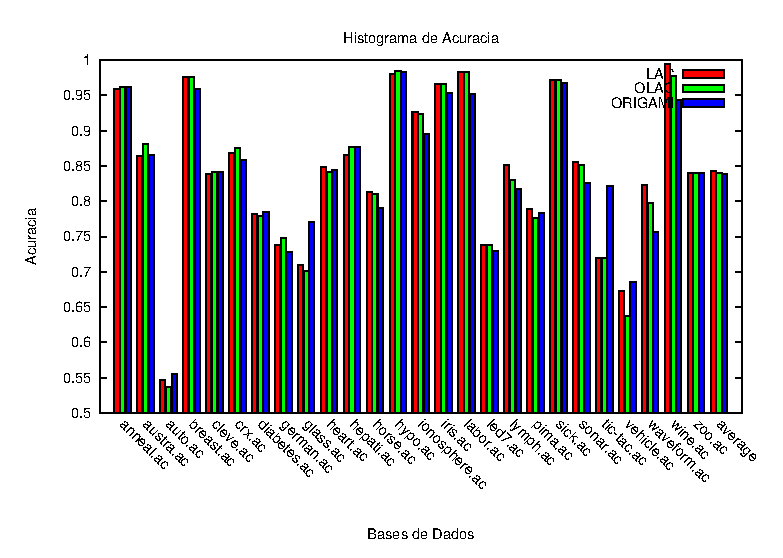
\includegraphics[width=\textwidth]{../thesis/graphs/histogram_best_run_for_each_db_acc}
	\end{centering}
\end{frame}

\begin{frame}[shrink]{Melhores Resultados para Cada Base}
	\begin{centering}
	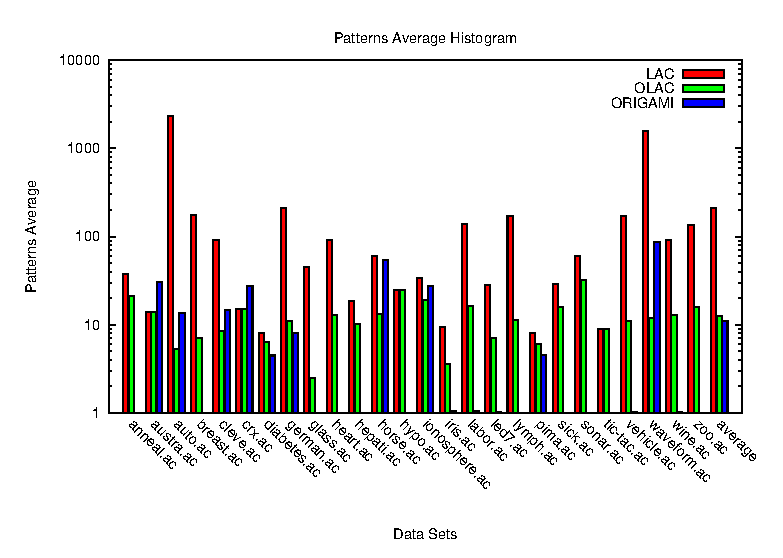
\includegraphics[width=\textwidth]{../thesis/graphs/histogram_best_run_for_each_db_pat}
	\end{centering}
\end{frame}

\begin{frame}[shrink]{Melhores Resultados para Cada Base}
	\begin{centering}
	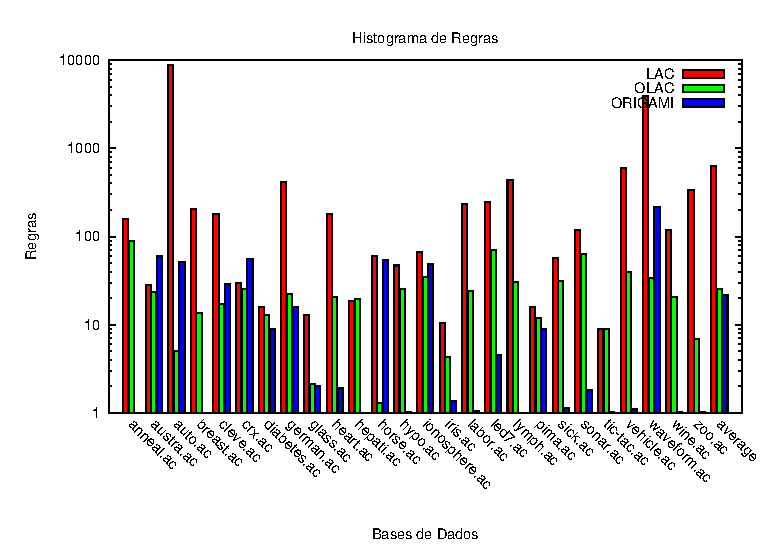
\includegraphics[width=\textwidth]{../thesis/graphs/histogram_best_run_for_each_db_rul}
	\end{centering}
\end{frame}

%\begin{frame}[shrink]{Melhores Resultados para Cada Base}
%	\begin{centering}
%	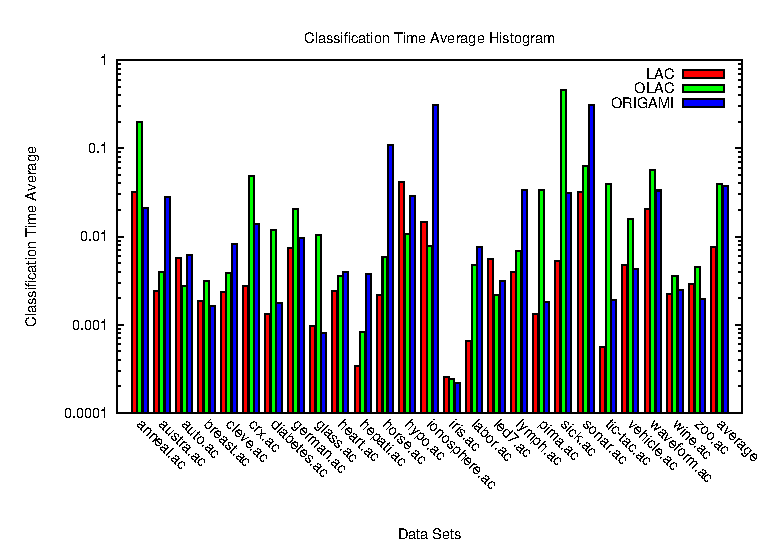
\includegraphics[width=\textwidth]{../thesis/graphs/histogram_best_run_for_each_db_tim}
%	\end{centering}
%\end{frame}

\begin{frame}[shrink]{Melhores M�dias dos Resultados para Todas as Bases}
	\begin{centering}
	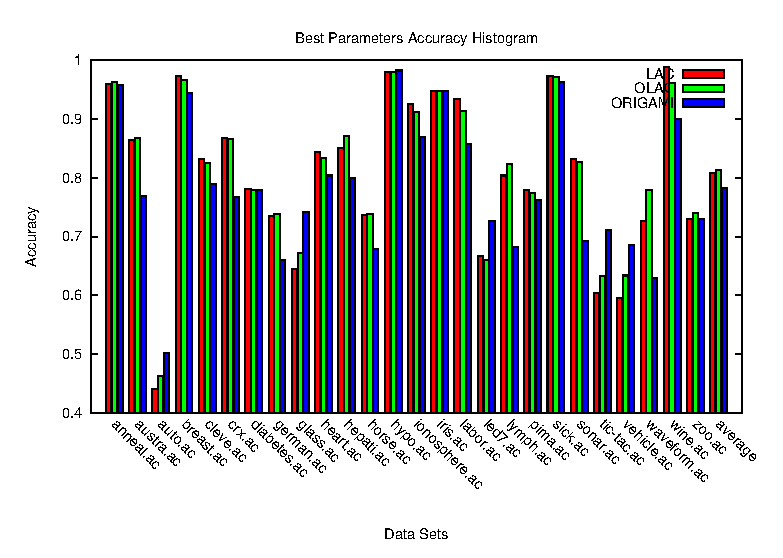
\includegraphics[width=\textwidth]{../thesis/graphs/histogram_best_run_for_avg_db_acc}
	\end{centering}
\end{frame}

\begin{frame}[shrink]{Melhores M�dias dos Resultados para Todas as Bases}
	\begin{centering}
	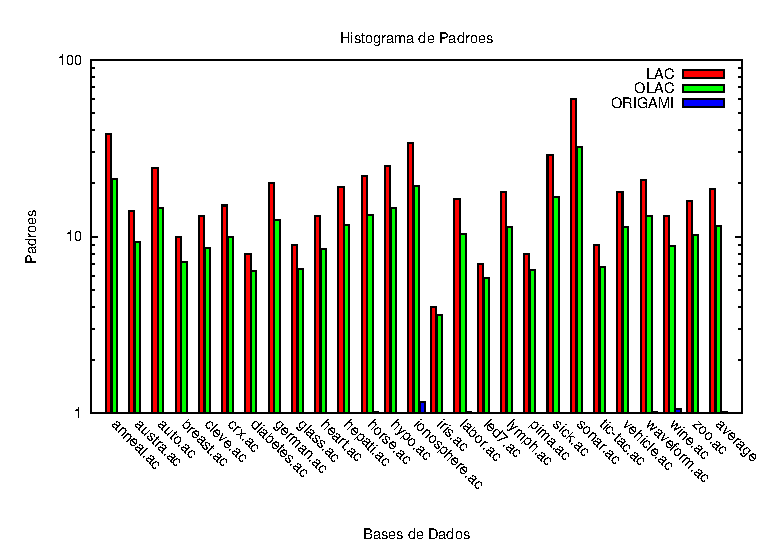
\includegraphics[width=\textwidth]{../thesis/graphs/histogram_best_run_for_avg_db_pat}
	\end{centering}
\end{frame}

\begin{frame}[shrink]{Melhores M�dias dos Resultados para Todas as Bases}
	\begin{centering}
	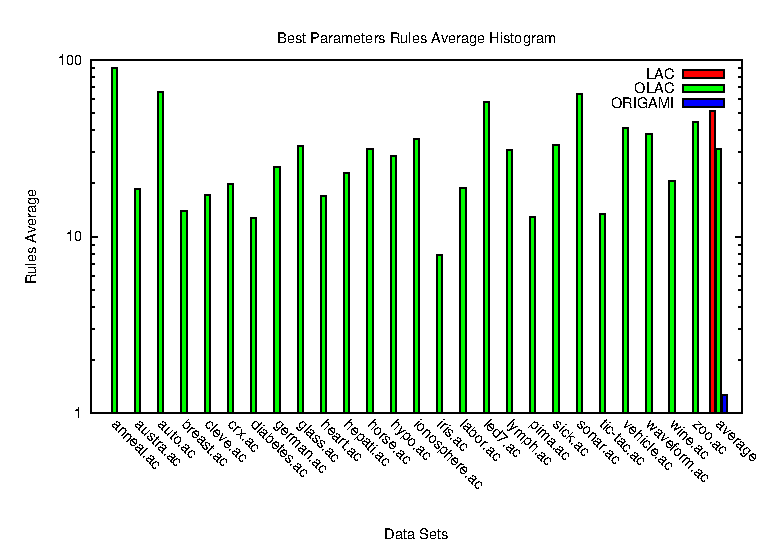
\includegraphics[width=\textwidth]{../thesis/graphs/histogram_best_run_for_avg_db_rul}
	\end{centering}
\end{frame}

% O Aplicativo olac
% Exemplo de Execu��o
% Experimentos
\chapter{Conclus�o}
\label{chapter:conclusao}

Neste trabalho foi explorado o conceito de ortogonalidade em minera��o de dados com o objetivo de se diminuir a redund�ncia e, conseq�entemente, o tamanho do conjunto de padr�es freq�entes de uma base de dados. A estrat�gia foi aplicada ao problema da classifica��o associativa, onde a ortogonalidade foi explorada sob tr�s perspectivas: estrutura dos padr�es, cobertura de transa��es e cobertura de classes.
\par
Foi implementado um classificador baseado em regras de associa��o com tr�s abordagens distintas: a abordagem cl�ssica \textbf{LAC} (\textit{Lazy Associative Classifier}), proposta em \cite{Veloso06Lazy}, que simplesmente obt�m, para cada inst�ncia de teste, um conjunto de padr�es freq�entes, e o utiliza para gerar regras associativas, a abordagem ortogonal \textbf{OLAC} (\textit{Orthogonal Lazy Associative Classifier}), que extrai, do conjunto de padr�es freq�entes, um sub-conjunto de padr�es ortogonais, e utiliza este sub-conjunto para gerar as regras de associa��o, e uma adapta��o do \textbf{ORIGAMI}, encontrado na literatura, e desenvolvido, originalmente, para obten��o de padr�es ortogonais em grafos.
\par
Os experimentos comprovam a qualidade dos padr�es obtidos, visto que os algoritmos baseados em ortogonalidade obtiveram resultados semelhantes aos da abordagem cl�ssica. Vimos que, apesar do LAC ter levado uma pequena vantagem na maior parte das bases, os resultados obtidos pelas abordagens ortogonais mantiveram a qualidade, fazendo com que as m�dias das acur�cias para as tr�s abordagens ficassem muito pr�ximas.
\par
Considerando, para cada abordagem, os conjuntos de par�metros de execu��o que obtiveram os melhores resultados para cada base de dados, as m�dias de acur�cia obtidas para as abordagens LAC, OLAC e ORIGAMI foram, respectivamente, $0.843$, $0.840$ e $ 0.839$. J� os valores m�dios para as quantidades de padr�es utilizados na gera��o das regras foram $213$ para o LAC, e $12$ para o OLAC e o ORIGAMI. Como conseq��ncia da diminui��o do conjunto de padr�es, o n�mero m�dio de regras geradas pelas abordagens OLAC e ORIGAMI foram, respectivamente, $25$ e $23$, enquanto o LAC gerou, em m�dia, $628$ regras para cada classifica��o.
\par
Nas execu��es realizadas com o conjunto de par�metros que obteve a melhor m�dia dos resultados, os resultados obtidos para as abordagens LAC, OLAC e ORIGAMI foram, respectivamente, $0.808$, $0.813$ e $0.782$. Os valores m�dios para as quantidades de padr�es utilizados na gera��o das regras foram, respectivamente, $19$, $12$ e $1$, e os valores m�dios para n�meros de regras geradas foram, respectivamente, $51$, $31$ e $1$.
\par
Para as abordagens ortogonais, notamos uma predomin�ncia da m�trica de ortogonalidade baseada na estrutura dos padr�es entre os par�metros de execu��o respons�veis pelos melhores resultados para cada base de dados. Vimos que as m�tricas baseadas em cobertura, tanto de classes quanto de transa��es, obtiveram conjuntos muito limitados, e compostos de padr�es, muitas vezes, pouco freq�entes. Isto fez com que tais m�tricas, mesmo diminuindo a ambiguidade das regras, n�o obtivessem resultados t�o bons quanto a baseada na estrutura dos padr�es.
\par
Vimos tamb�m que o ORIGAMI apresentou, em grande parte dos resultados, conjuntos ortogonais com apenas $1$ elemento. O motivo disto foram os baixos valores para suporte encontrados entre os par�metros de execu��o que obtiveram os melhores resultados para a maioria das bases.
\par
Tamb�m foram apresentados alguns casos de teste em que as abordagens ortogonais levaram desvantagem. Nestes casos, foi demonstrado que a falha na classifica��o n�o aconteceu por falta de qualidade nos conjuntos ortogonais, mas sim por causa das caracter�sticas dos padr�es ortogonais selecionados.
\par
Em resumo, vimos que a aplica��o de ortogonalidade no problema da classifica��o associativa possibilitou a minimiza��o do n�mero de padr�es utilizados na gera��o das regras, e, conseq�entemente, a diminui��o do conjunto de regras. Vimos tamb�m que, apesar de n�o obter melhores resultados com a diminui��o da ambiguidade, a ortogonalidade possibilitou a diminui��o da redund�ncia das regras geradas, mantendo a mesma qualidade dos resultados.

%Os resultados obtidos com a execu��o das tr�s abordagens considerando o melhor conjunto de par�metros para cada base de dados 

\section{Trabalhos Futuros}

Como trabalhos futuros, podemos citar a utiliza��o de ortogonalidade em outros pontos do algoritmo de classifica��o. Uma forma alternativa de se abordar o problema seria obter um sub-conjunto de itens ortogonais em rela��o � base de dados, a partir deste, obter todos os padr�es freq�entes que seriam considerados na gera��o das regras. Outra forma seria gerar todas as regras poss�veis a partir do conjunto de padr�es freq�entes, e aplicar a ortogonalidade, em conjunto com as demais medidas de interesse, na extra��o do sub-conjunto de regras consideradas para a classifica��o. Tamb�m seria interessante trabalhar em novas heur�sticas de obten��o de conjuntos ortogonais, com �nfase em desempenho, e investir no desenvolvimento de novos algoritmos de minera��o de padr�es freq�entes que j� considerem ortogonalidade durante a explora��o do espa�o de busca dos padr�es.
\par
A utiliza��o de uma abordagem h�brida OLAC-ORIGAMI tamb�m seria uma alternativa para tentar melhorar a acur�cia dos resultados. A nova abordagem faria uso dos par�metros $\alpha$ e $\beta$ aplicados ao conjunto de padr�es freq�entes, e n�o ao seu sub-conjunto de padr�es maximais. Esta solu��o seria �til para se obter conjuntos de padr�es ortogonais de melhor qualidade, j� que o usu�rio poderia controlar a medida de ortogonalidade e de representatividade da solu��o, e todos os padr�es freq�entes seriam candidatos ao conjunto ortogonal.


%\appendix
%\section{Exemplo de Execução da Heurística de Obtenção de Conjuntos Ortogonais}

\begin{frame}
	\begin{itemize}[<+-| alert@+>]
		\item $\F = \{A, B, BC, ABC\}$
		\item $Sort (\F)$
		\item $\F = \{ABC, BC, A, B\}$
	\end{itemize}
\end{frame}

\begin{frame}
	\begin{itemize}[<+-| alert@+>]
		\item $\F = \{ABC, BC, A, B\}$
		\item $Or = \{ABC, BC\}$
	\end{itemize}
\end{frame}

\begin{frame}
	\begin{itemize}[<+-| alert@+>]
		\item $\F = \{ABC, BC, A, B\}$
		\item $Or = \{ABC, BC\}$
	\end{itemize}
\end{frame}


\end{document}
